%%%%%%%%%%%%%%%%%%%%%%%%%%%%%%%%%%%%%%%%%
% Beamer Presentation
% LaTeX Template
% Version 1.0 (10/11/12)
%
% This template has been downloaded from:
% http://www.LaTeXTemplates.com
%
% License:
% CC BY-NC-SA 3.0 (http://creativecommons.org/licenses/by-nc-sa/3.0/)
%
%%%%%%%%%%%%%%%%%%%%%%%%%%%%%%%%%%%%%%%%%

%----------------------------------------------------------------------------------------
%	PACKAGES AND THEMES
%----------------------------------------------------------------------------------------

\documentclass{beamer}

\mode<presentation> {

% The Beamer class comes with a number of default slide themes
% which change the colors and layouts of slides. Below this is a list
% of all the themes, uncomment each in turn to see what they look like.

%\usetheme{default}
%\usetheme{AnnArbor}
%\usetheme{Antibes}
%\usetheme{Bergen}
%\usetheme{Berkeley}
\usetheme{Berlin}
%\usetheme{Boadilla}
%\usetheme{CambridgeUS}
%\usetheme{Copenhagen}
%\usetheme{Darmstadt}
%\usetheme{Dresden}
%\usetheme{Frankfurt}
%\usetheme{Goettingen}
%\usetheme{Hannover}
%\usetheme{Ilmenau}
%\usetheme{JuanLesPins}
%\usetheme{Luebeck}
%\usetheme{Madrid}
%\usetheme{Malmoe}
%\usetheme{Marburg}
%\usetheme{Montpellier}
%\usetheme{PaloAlto}
%\usetheme{Pittsburgh}
%\usetheme{Rochester}
%\usetheme{Singapore}
%\usetheme{Szeged}
%\usetheme{Warsaw}

% As well as themes, the Beamer class has a number of color themes
% for any slide theme. Uncomment each of these in turn to see how it
% changes the colors of your current slide theme.

%\usecolortheme{albatross}
%\usecolortheme{beaver}
%\usecolortheme{beetle}
%\usecolortheme{crane}
%\usecolortheme{dolphin}
%\usecolortheme{dove}
%\usecolortheme{fly}
%\usecolortheme{lily}
%\usecolortheme{orchid}
%\usecolortheme{rose}
%\usecolortheme{seagull}
%\usecolortheme{seahorse}
%\usecolortheme{whale}
%\usecolortheme{wolverine}

%\setbeamertemplate{footline} % To remove the footer line in all slides uncomment this line
%\setbeamertemplate{footline}[page number] % To replace the footer line in all slides with a simple slide count uncomment this line

%\setbeamertemplate{navigation symbols}{} % To remove the navigation symbols from the bottom of all slides uncomment this line
}

\usepackage{graphicx} % Allows including images
\usepackage{booktabs} % Allows the use of \toprule, \midrule and \bottomrule in tables
\usepackage{color}
\usepackage{mathrsfs}

% image directory
\graphicspath{{imgs/}}

% font
\usepackage{times}
\usefonttheme{professionalfonts}

% caption font size
\usepackage{caption}
\captionsetup{font={small}}

\usepackage{comment}
\usepackage{multirow}

\hypersetup{
  pdfauthor={Liu Weizhi},
  pdfpagemode=FullScreen,
  colorlinks={true}
}
%----------------------------------------------------------------------------------------
%	TITLE PAGE
%----------------------------------------------------------------------------------------

\title[Credit Scoring using Random Forests]{Credit Scoring using Random Forests} % The short title appears at the bottom of every slide, the full title is only on the title page

\author{Liu Weizhi, Ji Cheng, Tian Rong} % Your name
\institute[NJU] % Your institution as it will appear on the bottom of every slide, may be shorthand to save space
{
School of Management and Engineering, Nanjing University \\ % Your institution for the title page
\medskip
\textit{weizhiliu2009@gmail.com} % Your email address
}
\date{\today} % Date, can be changed to a custom date

\begin{document}
\small

\begin{frame}
\titlepage % Print the title page as the first slide
\end{frame}

\begin{frame}
\frametitle{Division of Tasks}
\begin{itemize}
	\item Liu Weizhi: coding
	\item Ji Cheng: gathering related materials, collecting data
	\item Tian Rong: designing beamer
\end{itemize}
\end{frame}

\begin{frame}
\frametitle{Overview} % Table of contents slide, comment this block out to remove it
\tableofcontents % Throughout your presentation, if you choose to use \section{} and \subsection{} commands, these will automatically be printed on this slide as an overview of your presentation
\end{frame}

%----------------------------------------------------------------------------------------
%	PRESENTATION SLIDES
%----------------------------------------------------------------------------------------
\section{introduction}

\subsection{Credit Risk Control Introduction}
%------------------------------------------
\begin{frame}
\frametitle{Cause of Credit Risk Control}
\begin{itemize}
	\item Credit card brings convenient to consumers as well as huge profit to the bank.
	\item However, high profits usually accompany with high risk.
	\item Banks, as the issuers of credit cards, undertake the potential risk.
\end{itemize}
\end{frame}

%------------------------------------------
\begin{frame}
\frametitle{The Development of Credit Risk Control}
\begin{itemize}
	\item The judgement is usually based on the experience of risk assessment experts.
	\item Find the customer with potential risk by statistical means.
	\item Use efficient data analysis tools and methods.
\end{itemize}
\end{frame}

%------------------------------------------
\begin{frame}
\frametitle{The Background of Credit Card}
\begin{itemize}
	\item First credit card appeared in March, 1995.
	\item The total number of credit cards reached at 1.22 hundred millions while the total number 
	      of credit card loans reached at 6931.73 hundred millions.
	\item Credit card brings convenient to consumers and huge profit to the bank high accompany with 
	      high risk.
\end{itemize}
\end{frame}

%------------------------------------------
\begin{frame}
\frametitle{The Background of Credit Card}
\begin{block}{Event}
Credit card companies which earned huge profit started to lose money at the same time as the high 
speed development in credit cards
\end{block}

Two main risks banks faced in China:
\begin{itemize}
	\item Credit Risks�� Issue credit cards by the means of  ``No Guarantee''
	\item Operational Risk
		  \begin{itemize}
			\item [--]Failure of internal control: Adopt aggressive marketing strategies because of the 
			      lack in knowledge of the credit card risk characteristics.
            \item [--]Transaction processing risk: Incomplete process and hacker attacks may easily happen.
		  \end{itemize}	
\end{itemize}
\end{frame}

%------------------------------------------
\begin{frame}
\frametitle{Means of Coping with Potential Risk}
Advanced technology and means is the fundamental guarantee to the development and security of credit card business. 
\begin{itemize}
	\item Self-built credit card business system and information system in China mostly were still in 
	      the stage of beginning, which cause the operational risk of credit cards. To solve these 
		  problems, the only method is to use the advanced technology to build a impeccable system.
    \item For instance, establishing modern authorization exchange network system and fund settlement 
	      system is the key to solving the problem of overdraft.
\end{itemize}
\end{frame}

\subsection{Meaning and Development of Credit Scoring}

%------------------------------------------
\begin{frame}
\frametitle{Meaning of Credit Scoring}
Credit scoring is a consuming credit managing technology which is widely used in Europe and the United States.
\begin{itemize}
	\item Based on Data Mining and Statistical Analysis.
	\item Building the predictive model.
	\item Making a comprehensive assessment of consumers' future performance with a credit score .
\end{itemize}
\end{frame}

%------------------------------------------
\begin{frame}
\frametitle{Role of credit rating}
Credit scoring model can provide credit managers with a large amount of highly predictive information.
\begin{itemize}
	\item Making effective management strategy
	\item Realizing high profit with the help of risk control
\end{itemize}
\end{frame}

%------------------------------------------
\begin{frame}
\frametitle{History of Credit Scoring}
\begin{itemize}
	\item The methods of diving the overall into several groups based on different characteristics 
	      was used by Fisher in1936 for the first time while David Durand firstly adopted this method 
		  to assess credit risk in 1941.
	\item Legislation which was named as ``Fair Credit Law'' and passed in the United States marked the
          fully acceptence to credit scores by the society.
	\item Credit scoring began to be adopted in other financial products by banks.
\end{itemize}
\end{frame}

%------------------------------------------
\begin{frame}
\frametitle{Classification of Credit Scoring}
\begin{itemize}
	\item Credit Scoring of Application \\
	      Focused on new applications for credit cards.
	\item Behavior Scoring \\
          Assessment in the probability of potential loss to Banks.
	\item Profit Scoring \\
		  Assessment in the potential profit which coming from card holders to Banks .
	\item Repayment Scoring \\
          Forecasting the effect of measures when bad loans appears
\end{itemize}
\end{frame}

%------------------------------------------
\begin{frame}
\frametitle{Advantages of Credit Scoring}
\begin{itemize}
	\item Objectivity: Based on huge amount of data.
	\item Consistency: Credit Scoring Model remain consistent during the process.
	\item Accuracy: Based on law of large number and statistical technology.
	\item Comprehensiveness: Credit Scoring Model is consisted of several predictor variables which 
	      represent all dimensions of Information .
	\item Efficiency: Decisions can be made within a few seconds.
\end{itemize}
\end{frame}

\subsection{Data Mining in Credit Card Industry}

%------------------------------------------
\begin{frame}
\frametitle{Market development and customer maintenance}
\begin{itemize}
	\item Customer segmentation model \\
          Separating customers in accordance with the different research purposes.
	\item Customers activate model \\
          Solving the problems caused by sleeping cards.
	\item Customer leaving model \\
          Preventing customers from running away.
\end{itemize}
\end{frame}

%------------------------------------------
\begin{frame}
\frametitle{Risk Control}
\begin{itemize}
	\item Applying Scoring Model \\
          Determining the line of credit.
	\item Behaving Scoring Model \\
          Assessment in the probability of happening of bad loans .
	\item Fraud Detecting Model \\
          Identifying fraudulent trading by analyzing the history of every customer.
\end{itemize}
\end{frame}

%------------------------------------------
\begin{frame}
\frametitle{\small Process of building Credit Scoring Model based on Data Mining}
\begin{figure}
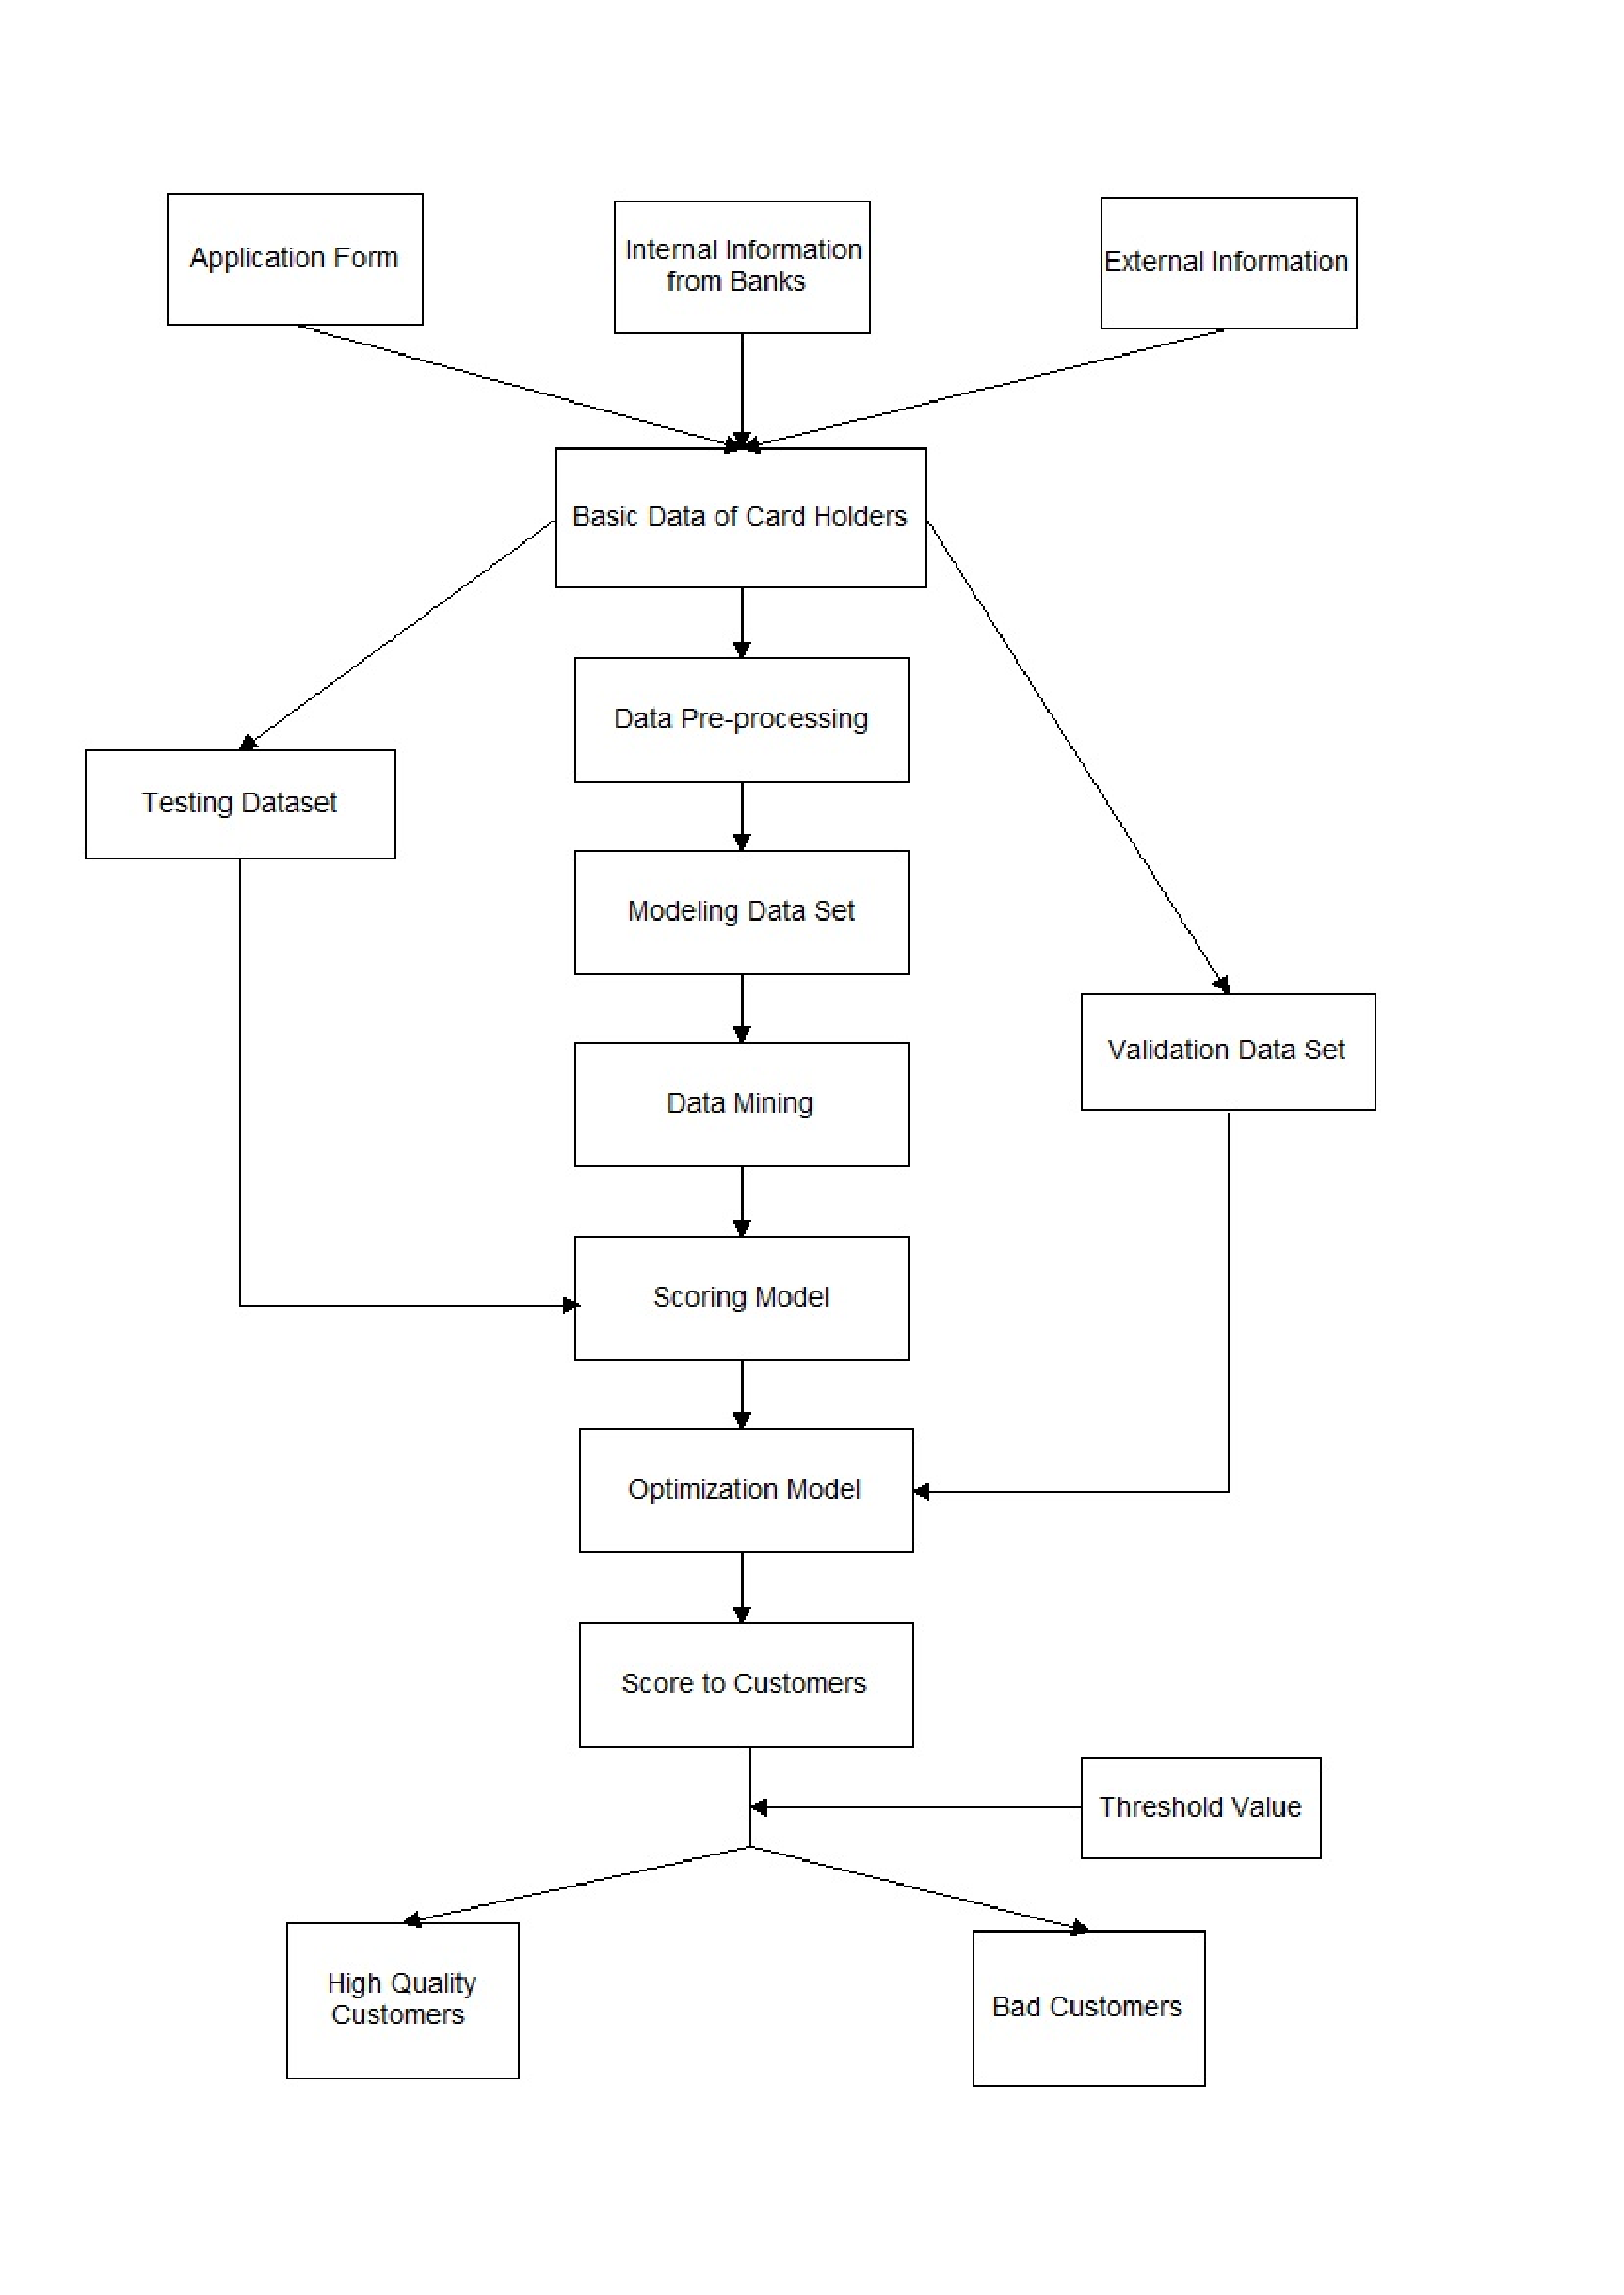
\includegraphics[width=0.4\linewidth]{flow.pdf}
\end{figure}
\end{frame}

%------------------------------------------
\begin{frame}
\frametitle{Our Goal}
We don't insist on calculating the specific credit score but to {\color{red}help the lenders to decide whether an application will turn into a bad loan in the future.}

Our basic idea is using three machine leaning methods, namely {\color{red}logistics regression, classification tree and 
random forests,} to predict whether borrowers will have a delinquency. The performance of each classifiers is 
compared using the test data set.

\begin{figure}

\includegraphics[width=0.6\linewidth]{fraud.pdf}
\end{figure}
\end{frame}

\section{data}
%------------------------------------------
\subsection{data source}
\begin{frame}
\frametitle{Data Source}
\begin{itemize}
	\item {\color{red} Bad loans are defined as those loans where repayments are not being made as originally agreed 
	      (eg. specific due date).}
	\item Two data sets were collected, one is German Credit, and another is from Kaggle.com.
	\item German Credit, including 1000 records whose 30\% are bad loans, was retrieved from UCI machine learning repository.
	\item Another data set was retrieved from Kaggle's competition "Give me Some Credit" which has 250,000
          records and 6.7\% bad loans. (We only used the first 10,000 records due to the lack of computation ability.)
\end{itemize}
\begin{columns}[c]
\column{0.45\textwidth}
\begin{figure}

\includegraphics[width=0.4\linewidth]{uci.pdf}
\end{figure}
\column{0.45\textwidth}
\begin{figure}

\includegraphics[width=0.4\linewidth]{kaggle.pdf}
\end{figure}
\end{columns}
\end{frame}
%------------------------------------------
\subsection{data description}
\begin{frame}
\frametitle{Data Description}
Take German Credit as example. German Credit consists of 21 columns whose first column indicates whether 
a loan was good or bad. The next 20 features are as follows: {\color{red}checking, duration, history, purpose, 
amount, savings, employ, installment, status, others, residence, property, age, otherplans, housing, 
cards, job, liable, tele, foreign.} Some features are represented by the specific codes like `A34', `A32', etc.
\begin{figure}
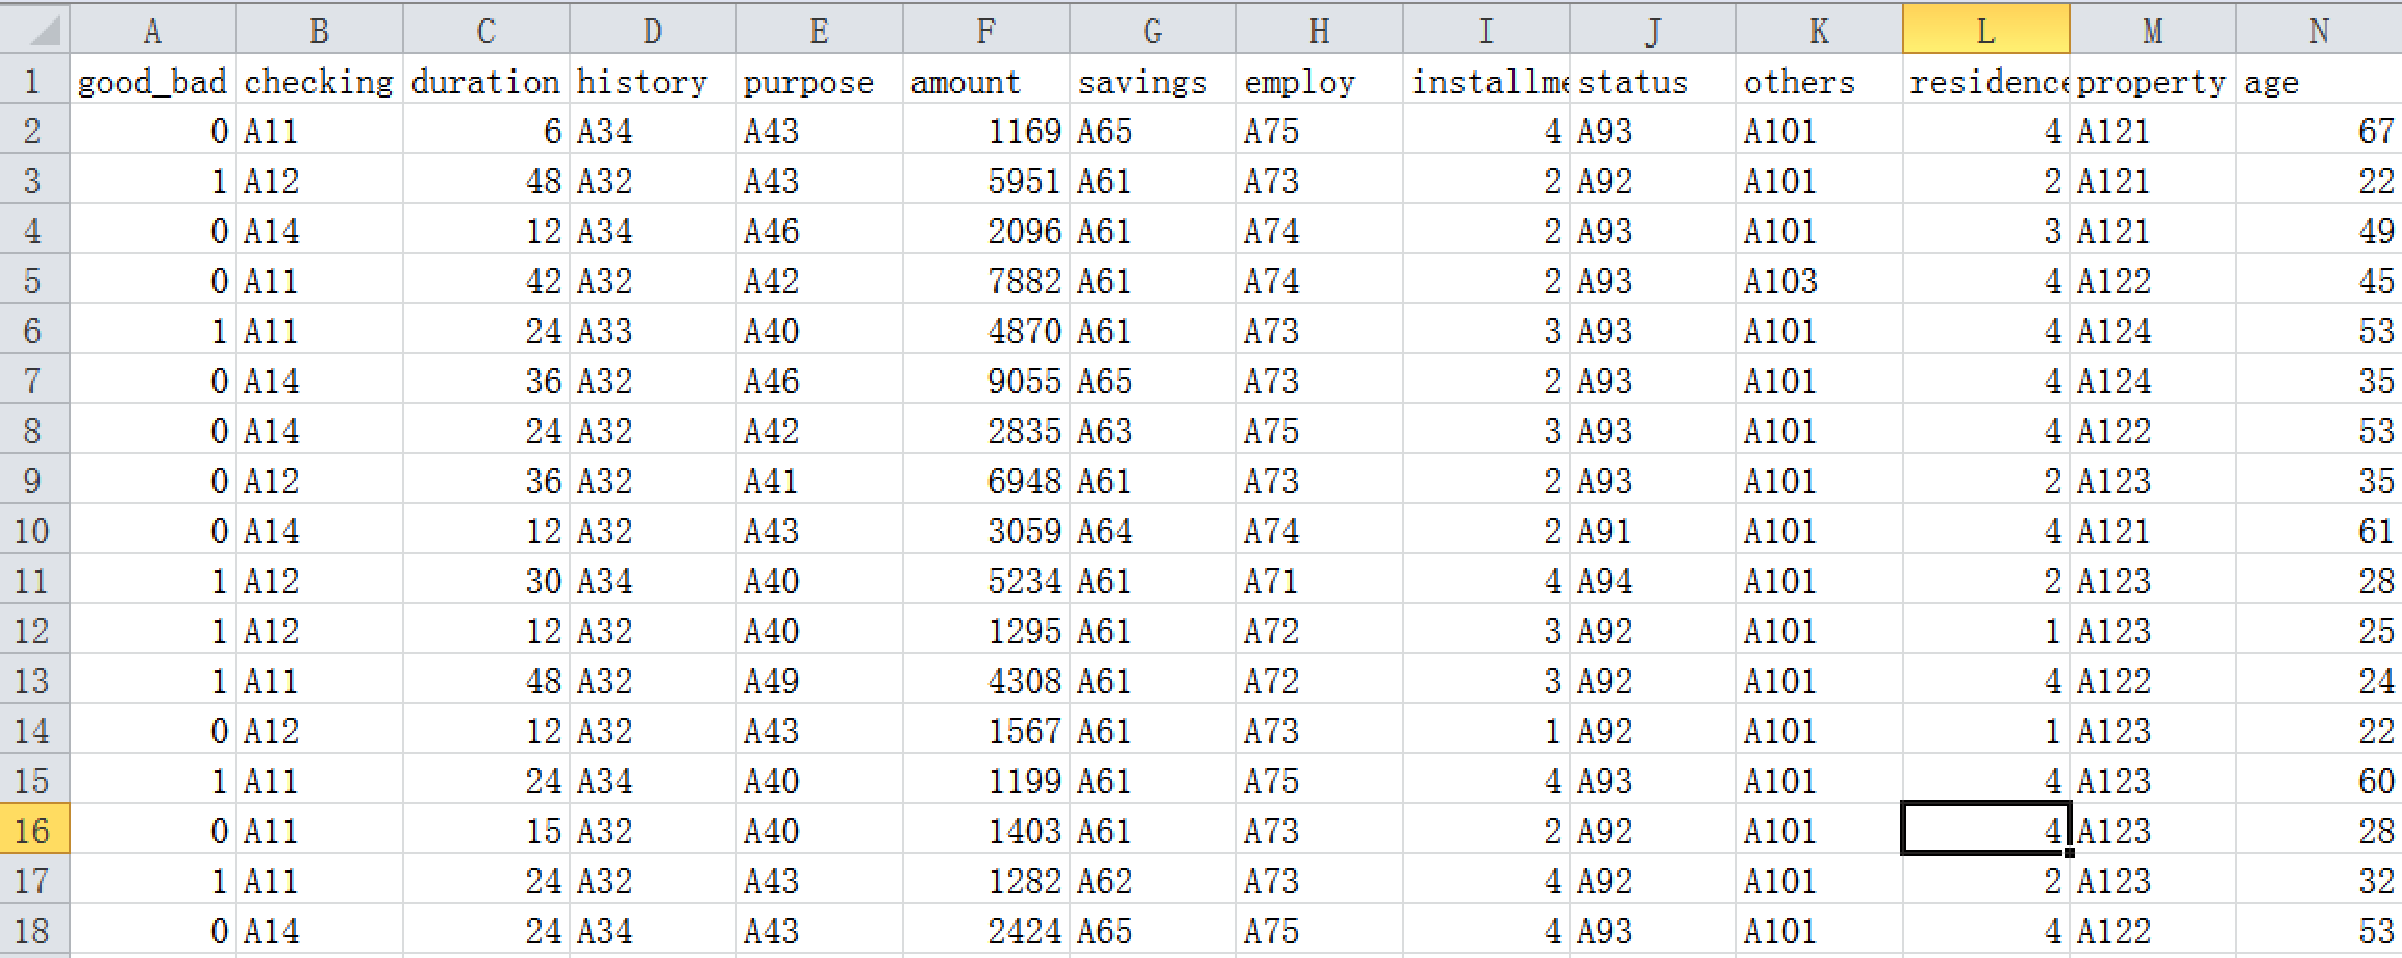
\includegraphics[width=0.8\linewidth]{germandata.pdf}
\end{figure}
\end{frame}

\section{methods}
\subsection{logistic regression}
%------------------------------------------
\begin{frame}
\frametitle{Logistic Regression Introduction}
\begin{itemize}
	\item Assuming a linear regression $y = \theta x$, where $x$ is the feature vector and $\theta$ is 
          the corresponding parameters.
	\item However, the value of $y$ might range widely in the real space, which is not appropriate for the 
	      classification problems in which $y$ belongs to a discrete set, like \{'Positive Class', 'Negative Class'\}.
	\item Logistic Regression adopts logistic function, which can be applied to depict the probability of 
	      some events.
\end{itemize}

\end{frame}

%------------------------------------------
\begin{frame}
\frametitle{Logistic Regression Algorithm}
\begin{itemize}
	\item Logistic Function: {\color{red}$h(z) = \frac{1}{1+e^{-z}}$, let $z=\theta x$, then $h(\theta x) = \frac{1}{1+e^{-\theta x}} \in [0, 1]$.}
	\item Cost Function: {\color{red}$cost(\theta) = - y log(h(\theta x)) - (1-y) log(1-h(\theta x))$.} Minimize this function to estimate the parameters $\theta$.
\end{itemize}

\begin{columns}[c]
\column{0.45\textwidth}
\begin{figure}
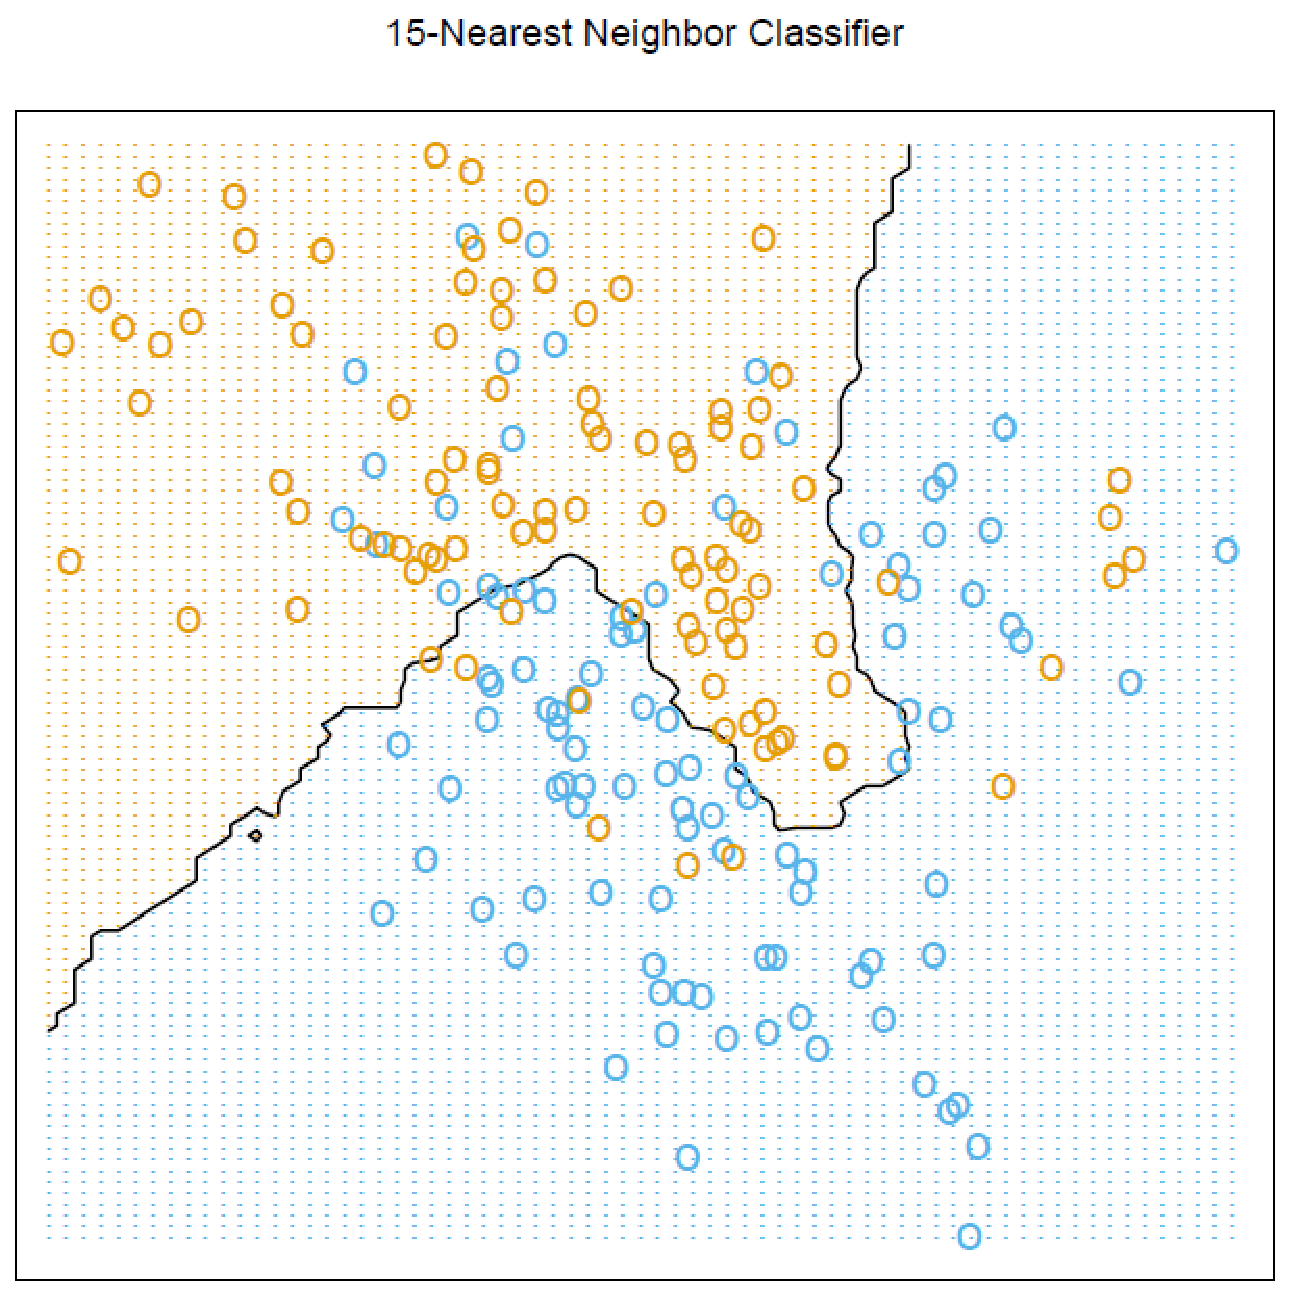
\includegraphics[width=0.5\linewidth]{bound.pdf}
\caption{Decision Boundary}
\end{figure}
\column{0.45\textwidth}
\begin{figure}
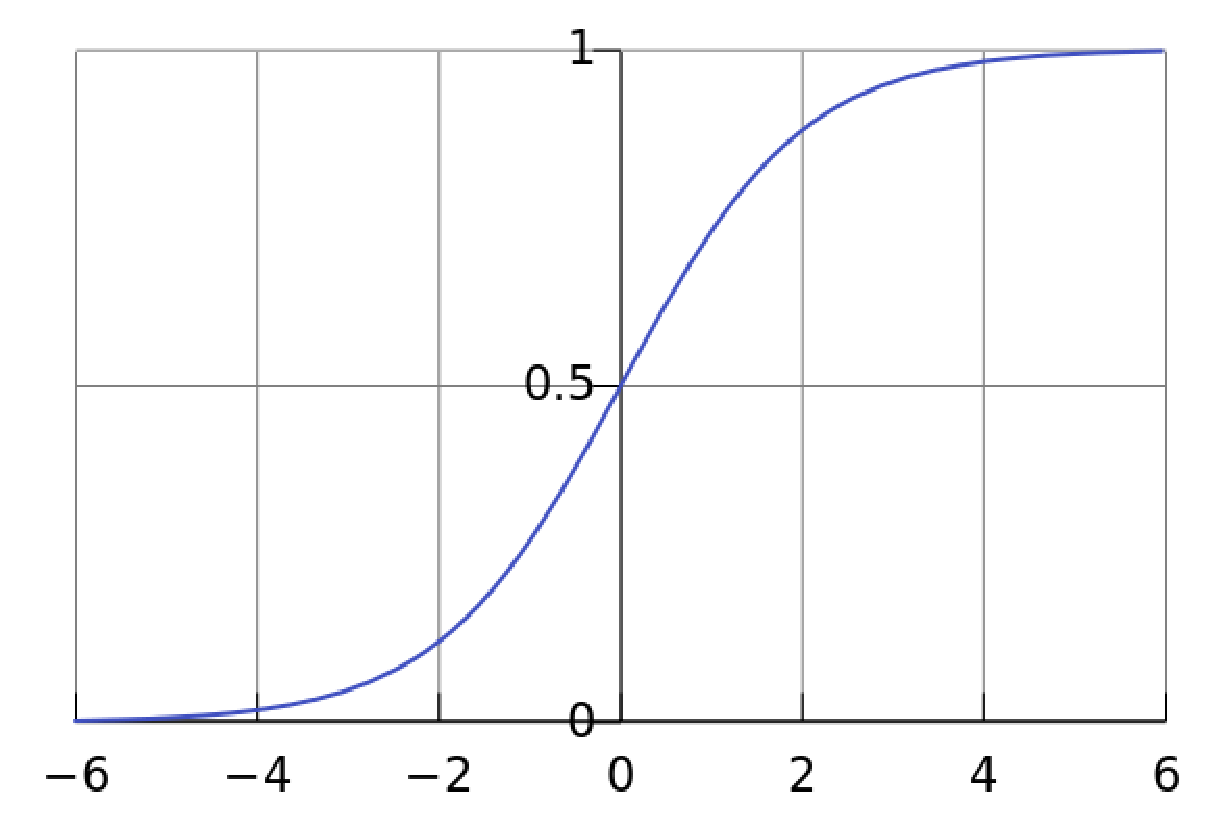
\includegraphics[width=0.7\linewidth]{logit.pdf}
\caption{Logistic Function}
\end{figure}
\end{columns}
\end{frame}

%------------------------------------------
\begin{frame}
\frametitle{Logistic Regression Results}
\tiny
% Table generated by Excel2LaTeX from sheet 'logistic'
\begin{table}[htbp]
  \centering
    \begin{tabular}{lllll}
    \toprule
          & Estimate & Std. Error & z value & $Pr(\ge\|z\|)$ \\
    \midrule
    (Intercept) & -5.48743 & 1.387014 & -3.95629 & 7.61E-05 ***\\
    checking & 0.484832 & 0.089609 & 5.41055 & 6.28E-08 ***\\
    duration & -0.01426 & 0.01144 & -1.24679 & 0.212473 \\
    history & 0.469549 & 0.114837 & 4.088823 & 4.34E-05 ***\\
    purpose & 0.068907 & 0.042475 & 1.622316 & 0.104736 \\
    amount & -0.00015 & 5.07E-05 & -2.99869 & 0.002711 ***\\
    savings & 0.25071 & 0.076253 & 3.287871 & 0.001009 ***\\
    employed & 0.109647 & 0.095728 & 1.145409 & 0.25204 \\
    installp & -0.33189 & 0.106943 & -3.10348 & 0.001913 ***\\
    marital & 0.48904 & 0.155785 & 3.139197 & 0.001694 ***\\
    coapp & 0.100784 & 0.225263 & 0.447406 & 0.654582 \\
    resident & -0.10415 & 0.101927 & -1.02184 & 0.306856 \\
    property & -0.14986 & 0.12051 & -1.24353 & 0.213674 \\
    age   & 0.019083 & 0.011009 & 1.73332 & 0.083039 *\\
    other & 0.325128 & 0.140454 & 2.314837 & 0.020622 **\\
    housing & 0.274481 & 0.216319 & 1.268869 & 0.204488 \\
    existcr & -0.39916 & 0.203087 & -1.96544 & 0.049364 **\\
    job   & 0.34085 & 0.179191 & 1.902159 & 0.057150 *\\
    depends & -0.24825 & 0.290759 & -0.8538 & 0.393214 \\
    telephon & 0.021655 & 0.244287 & 0.088645 & 0.929364 \\
    foreign & 1.699978 & 0.891746 & 1.906348 & 0.056605 *\\
    \bottomrule
    \end{tabular}%
  \label{tab:logit}%
\end{table}%
\end{frame}
%------------------------------------------
\begin{frame}
\frametitle{Top 3 Reasons for Denial}
\begin{figure}
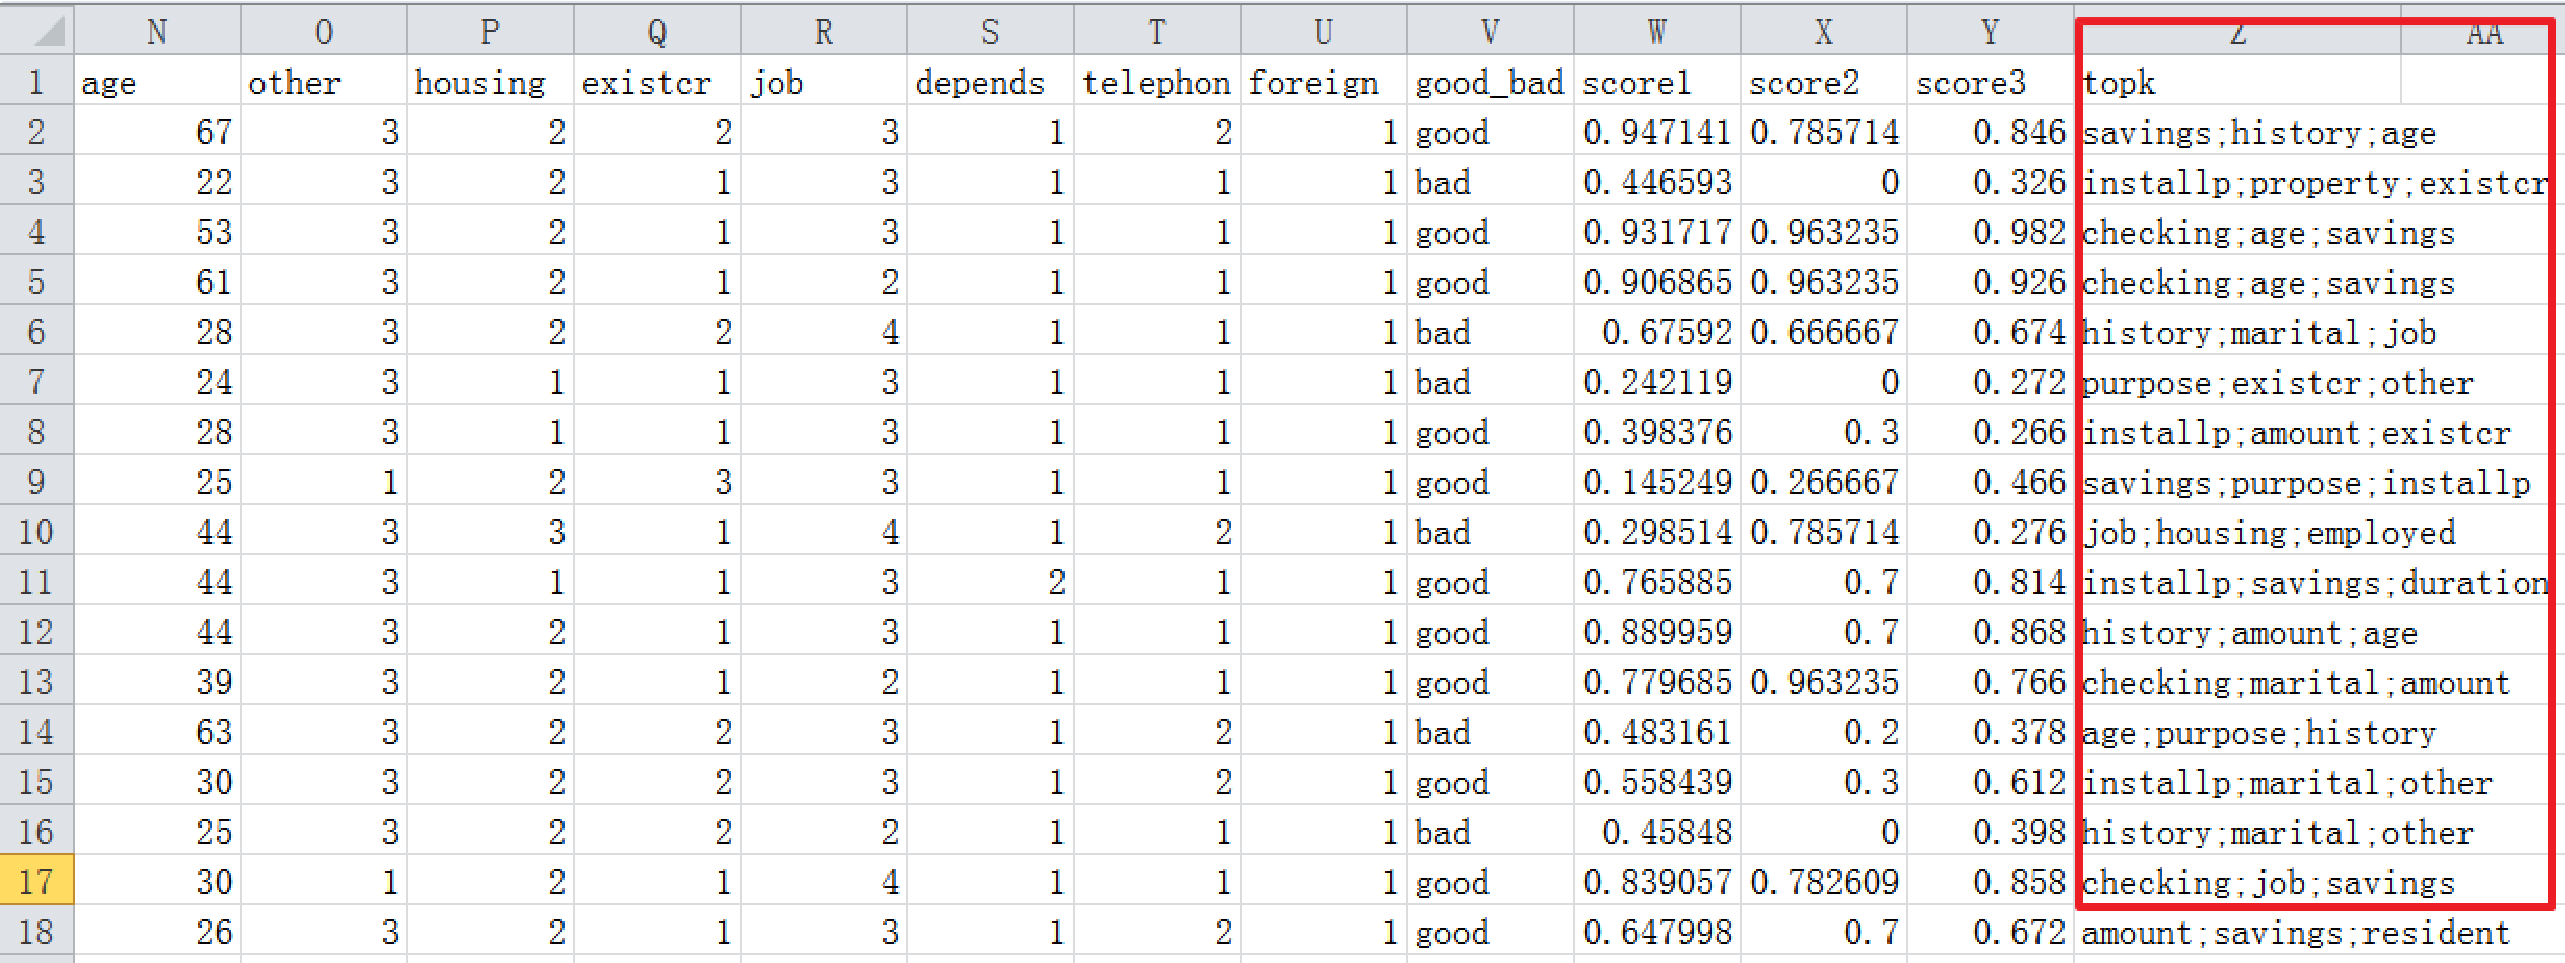
\includegraphics[width=1\textwidth]{topk.pdf}
\end{figure}
\end{frame}

\subsection{classification tree}
%------------------------------------------
\begin{frame}
\frametitle{Classification Tree Introduction}
\begin{columns}[c]
\column{0.3\textwidth}
\begin{figure}
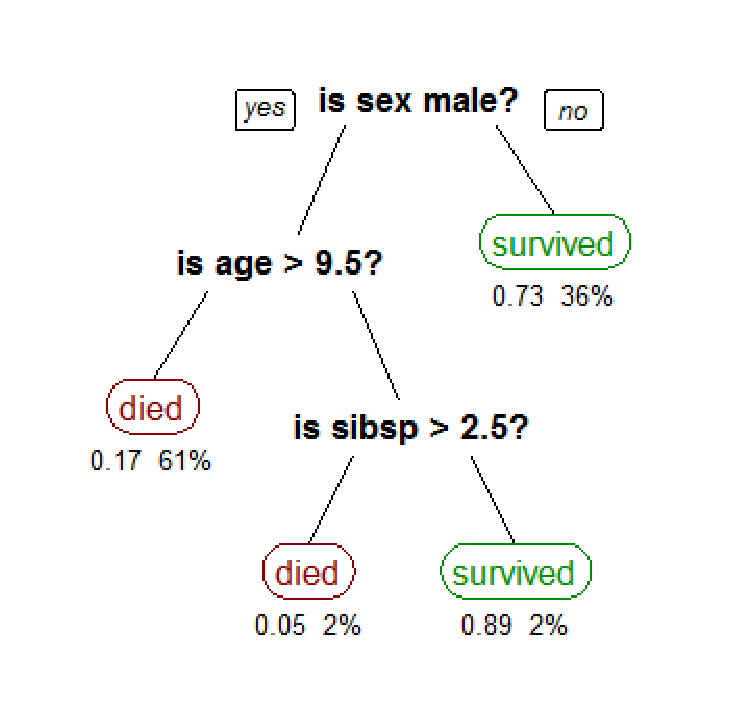
\includegraphics[width=1.2\linewidth]{titanic.pdf}
\caption{Titanic Survival Tree}
\end{figure}

\column{0.7\textwidth}
\begin{itemize}
	\item Decision tree learning uses a decision tree as a predictive model which maps observations 
	      about an item to conclusions about the item's target value.
	\item {\color{red}In these tree structures, leaves represent class labels and branches represent conjunctions 
	      of features that lead to those class labels.}
	\item The core of classification tree is to split father node to {\color{red}make the children node's subset more
	      pure} which can be depicted by \textbf{entropy}.
\end{itemize}
\end{columns}
\end{frame}

%------------------------------------------
\begin{frame}
\frametitle{Classification Tree ID3 Algorithm}
\begin{columns}[c]
\column{0.3\textwidth}
\begin{figure}
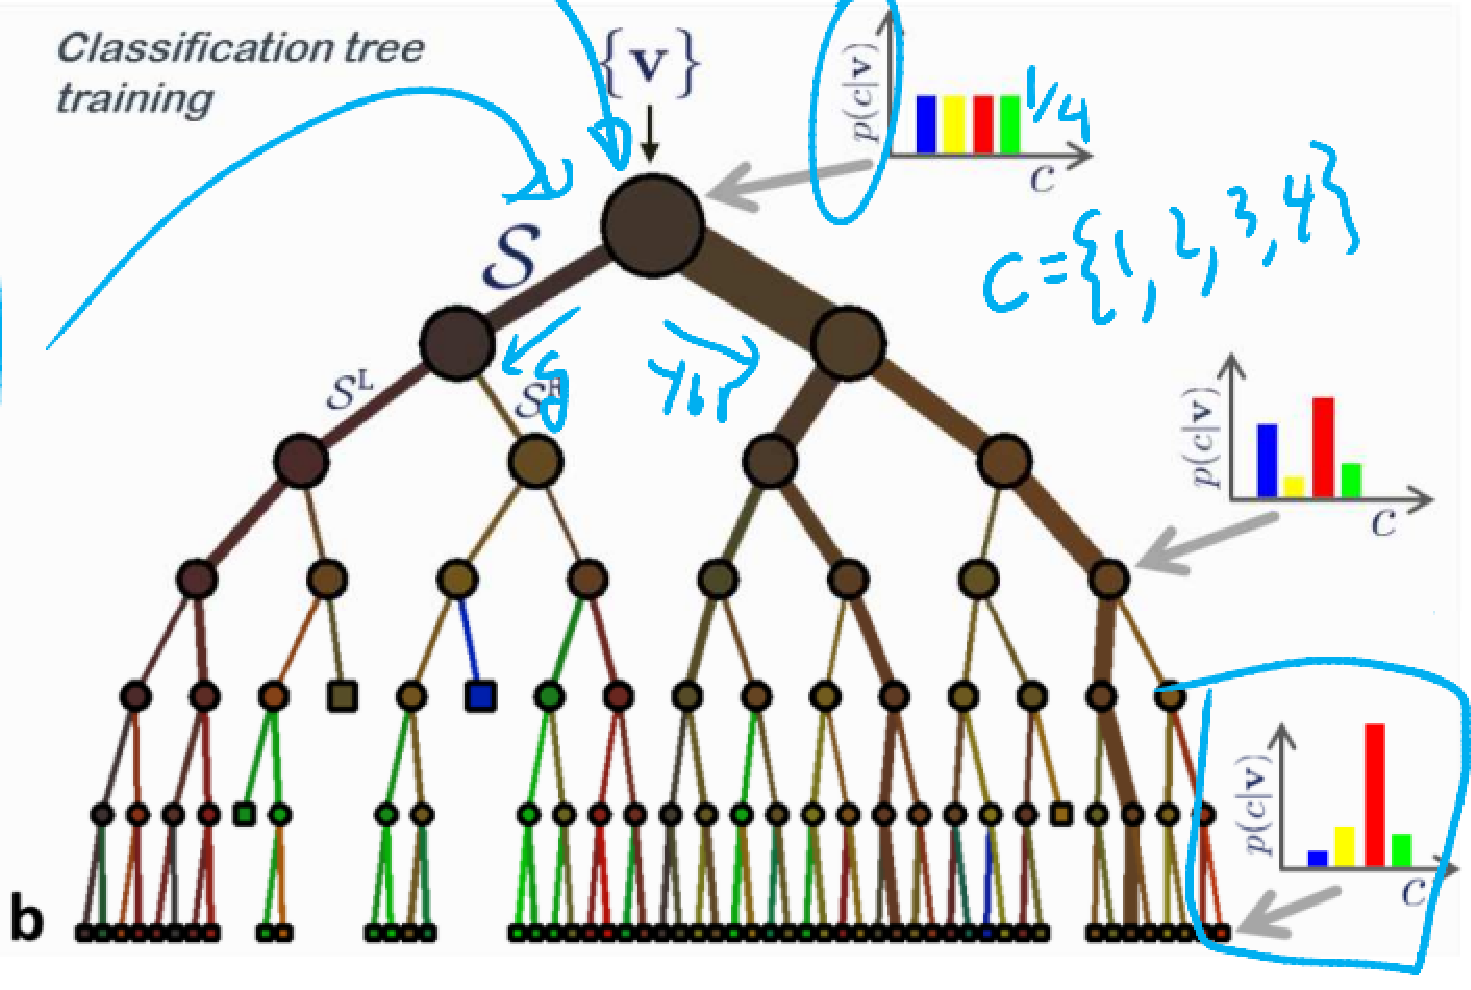
\includegraphics[width=1.2\linewidth]{entropy.pdf}
\caption{Classification Tree Entropy}
\end{figure}
\column{0.8\textwidth}
\begin{itemize}
	\item Entropy: The purity of subset $S$ can be calculated by {\color{red}$H(S) = - \sum _{i} p(i) log(p(i))$, }
	      where $p_{i}$ is the frequency of class $i$ in $S$. If there is only one class in the set 
		  $S$, then the entropy is 0.
	\item Information Gain: IG is the measure of difference in entropy between the original set $S$ and sets $T$ splited on attribute $\mathscr{Y}$. {\color{red}$IG(\mathscr{Y}) = H(S) - \sum_{i \in T} p(i) log(p(i))$}
	\item Select the splitting attribute which shares the highest information gain.
\end{itemize}
\end{columns}
\end{frame}
%------------------------------------------
\begin{frame}
\frametitle{Classification Tree Results}
\begin{figure}
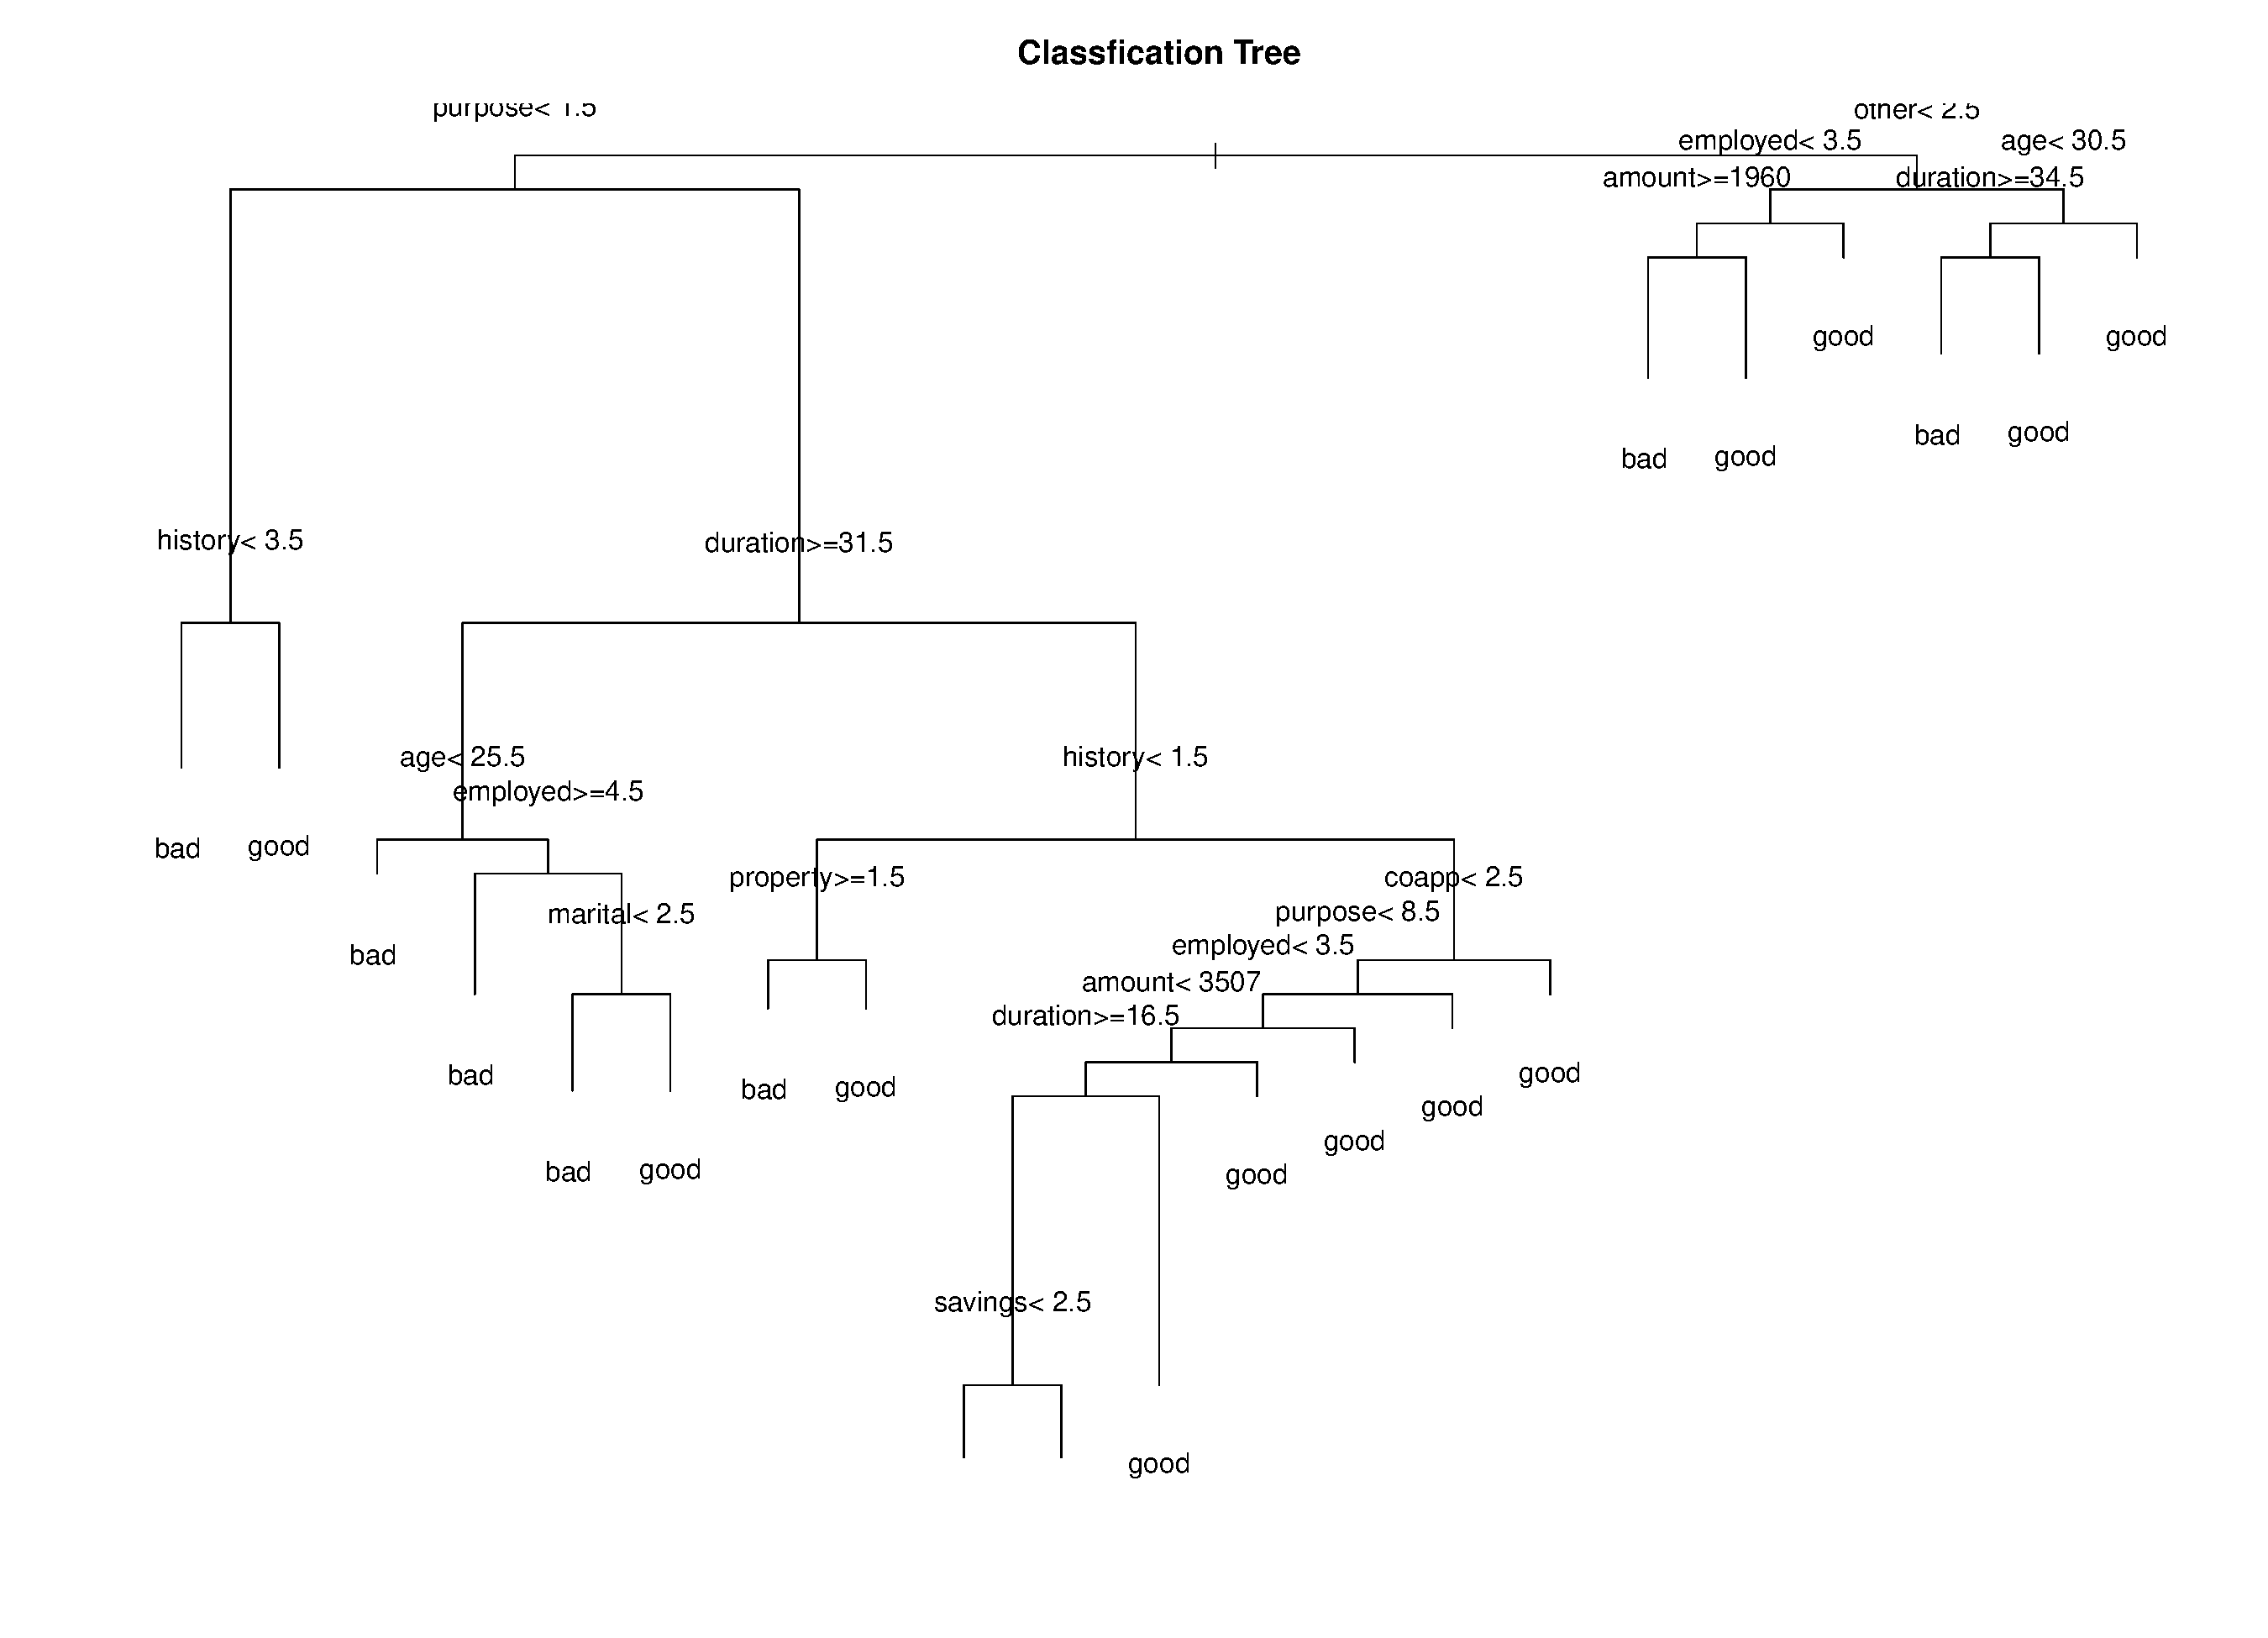
\includegraphics[width=0.8\textwidth]{classificationtree.pdf}
\end{figure}
\end{frame}
\subsection{random forests}
%------------------------------------------
\begin{frame}
\frametitle{Random Forests Introduction}
\begin{itemize}
	\item Random forests are an ensemble learning method for classification (and regression) that operate by constructing a multitude of decision trees at training time and outputting the class that is the mode of the classes output by individual trees.
	\item {\color{red}The most powerful aspect about random forests is variable importance ranking which estimates 
	      the predictive value of variables by scrambling the variable and seeing how much the model 
		  performance drops.}
	\item Kinect has used the random forests to detect humans' body movement.
\end{itemize}
\end{frame}

%------------------------------------------
\begin{frame}
\frametitle{Random Forests - Random Features}
\begin{columns}[c]
\column{0.6\textwidth}
\begin{figure}
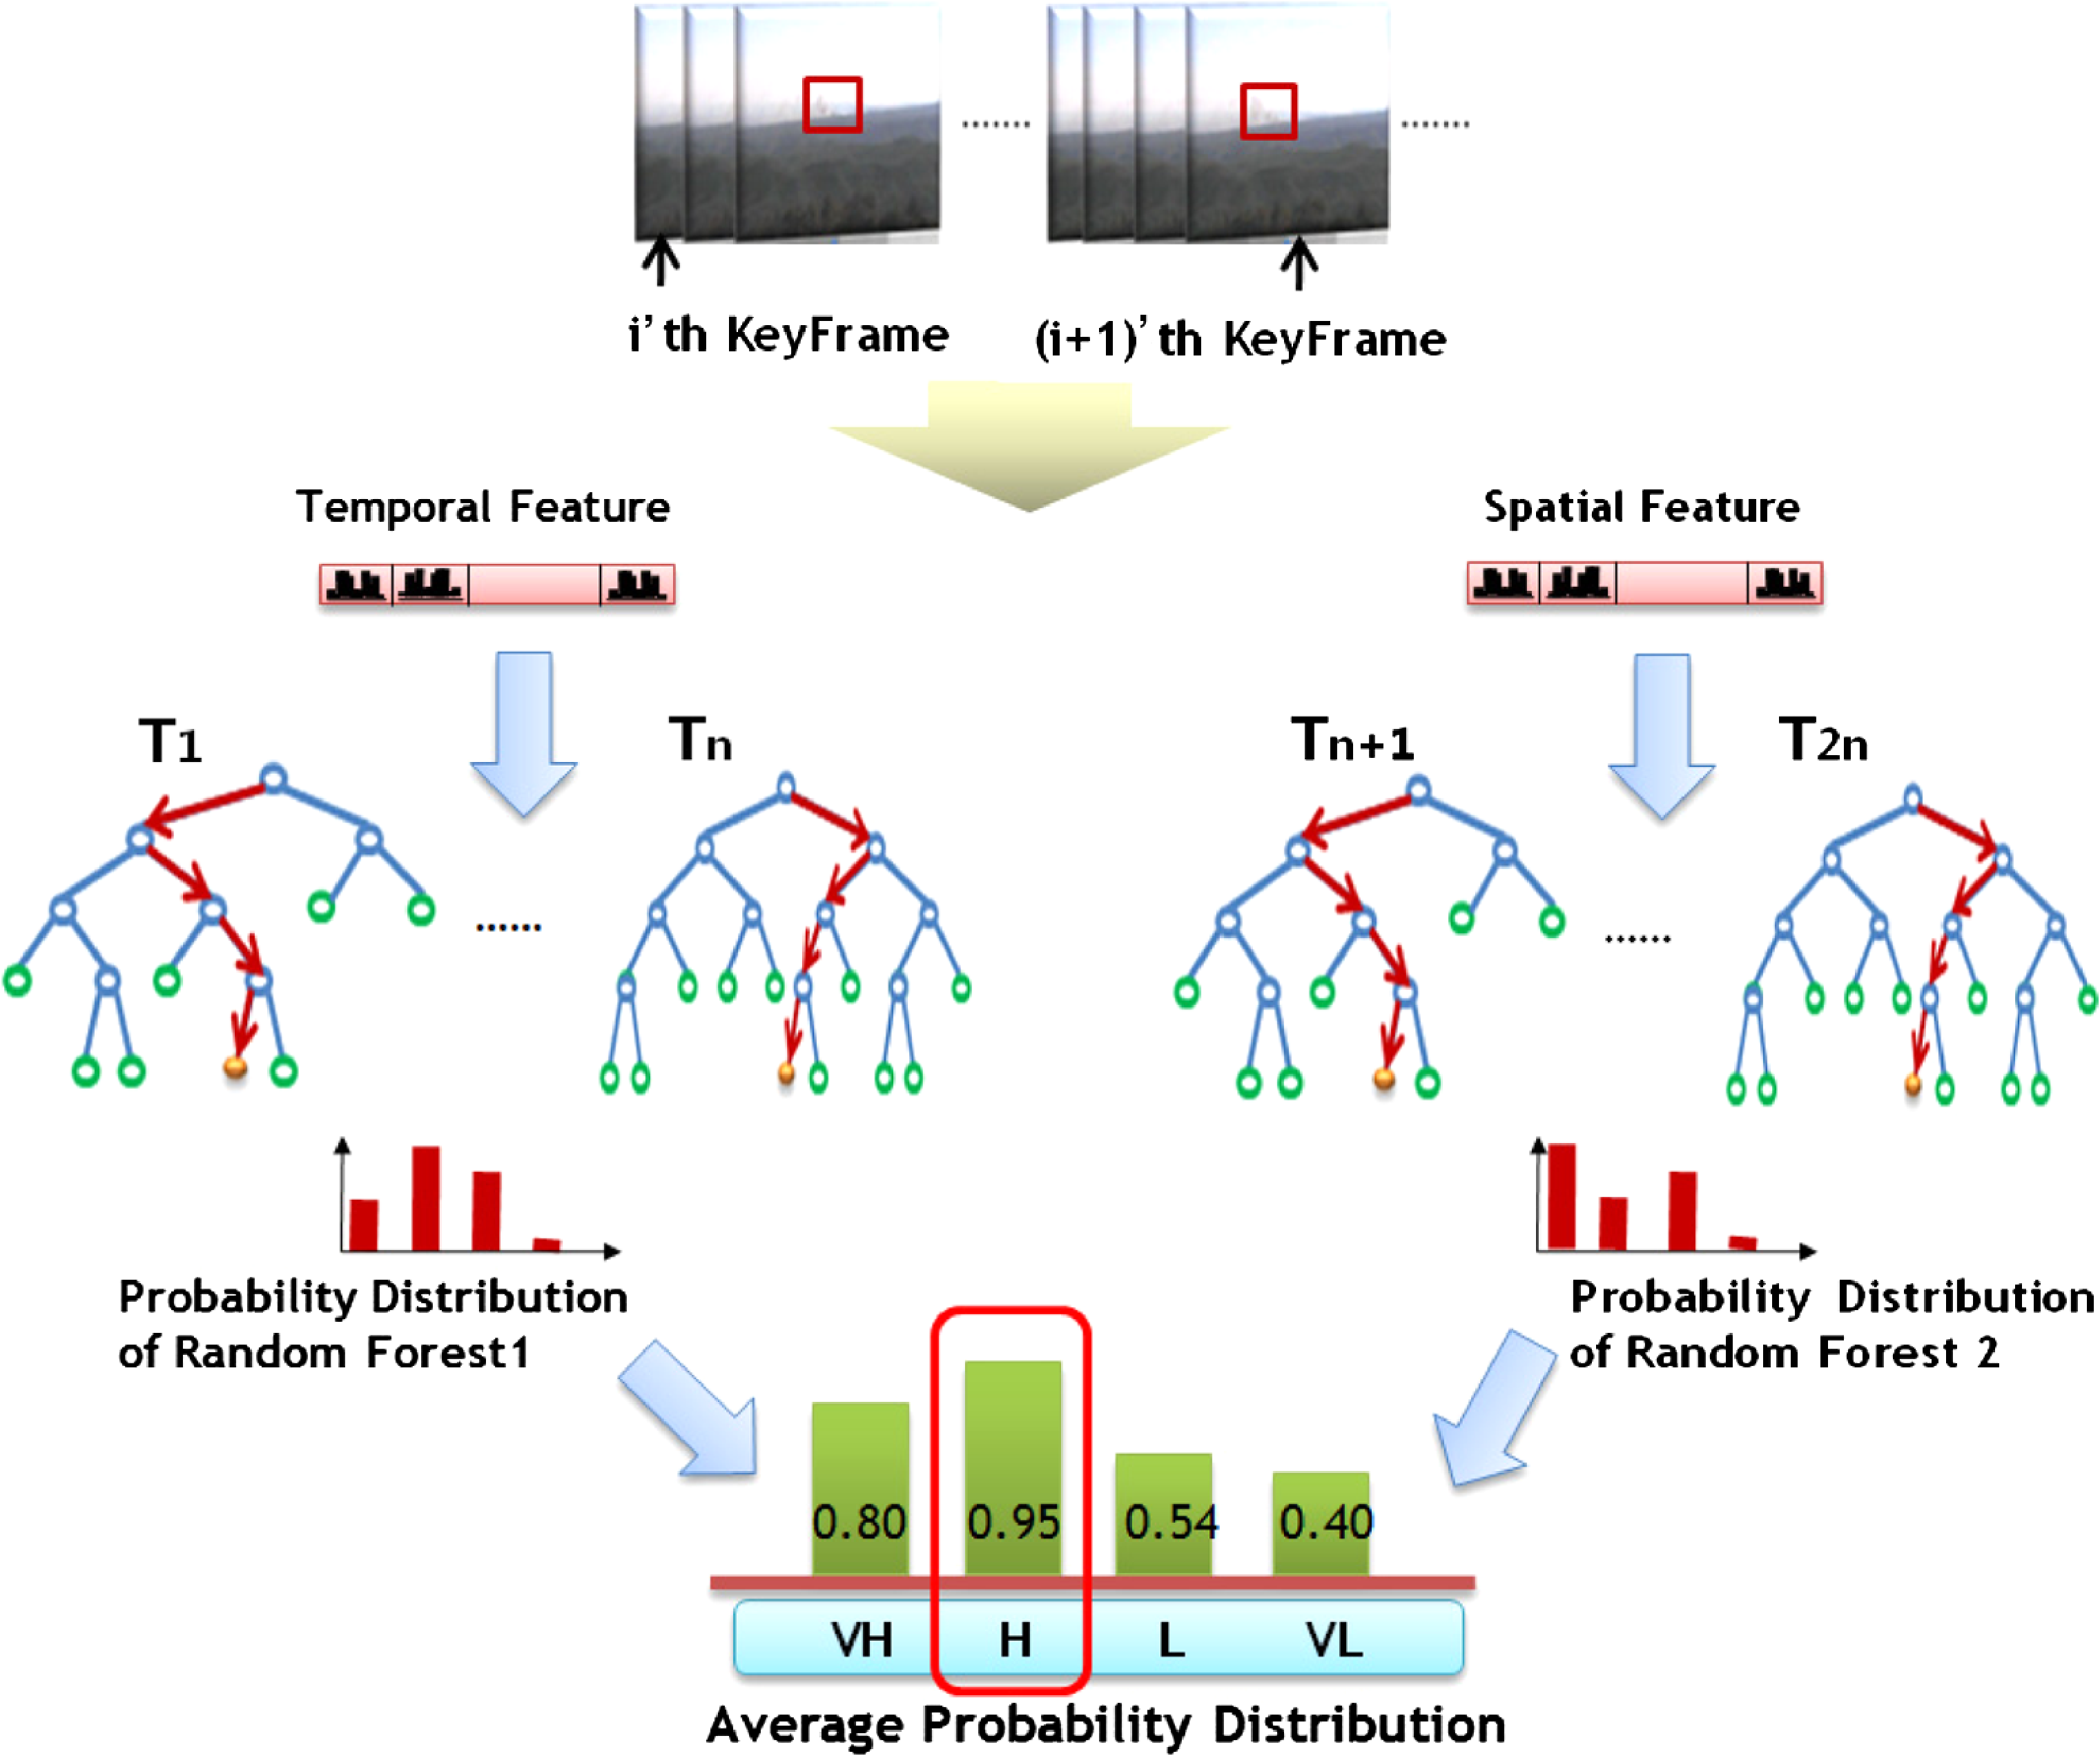
\includegraphics[width=0.8\linewidth]{rf.pdf}
\caption{Random Forests Algorithm }
\end{figure}
\column{0.5\textwidth}
\begin{itemize}
	\item Random Forests: The forests consist of many trees whose data set is {\color{red}the random bootstrap resampling} of original data.
	\item Random Features: Each tree shares {\color{red}a random subset feature} of original feature set.
\end{itemize}
\end{columns}
\end{frame}

%------------------------------------------
\begin{frame}
\frametitle{Variable Importance}
\begin{figure}
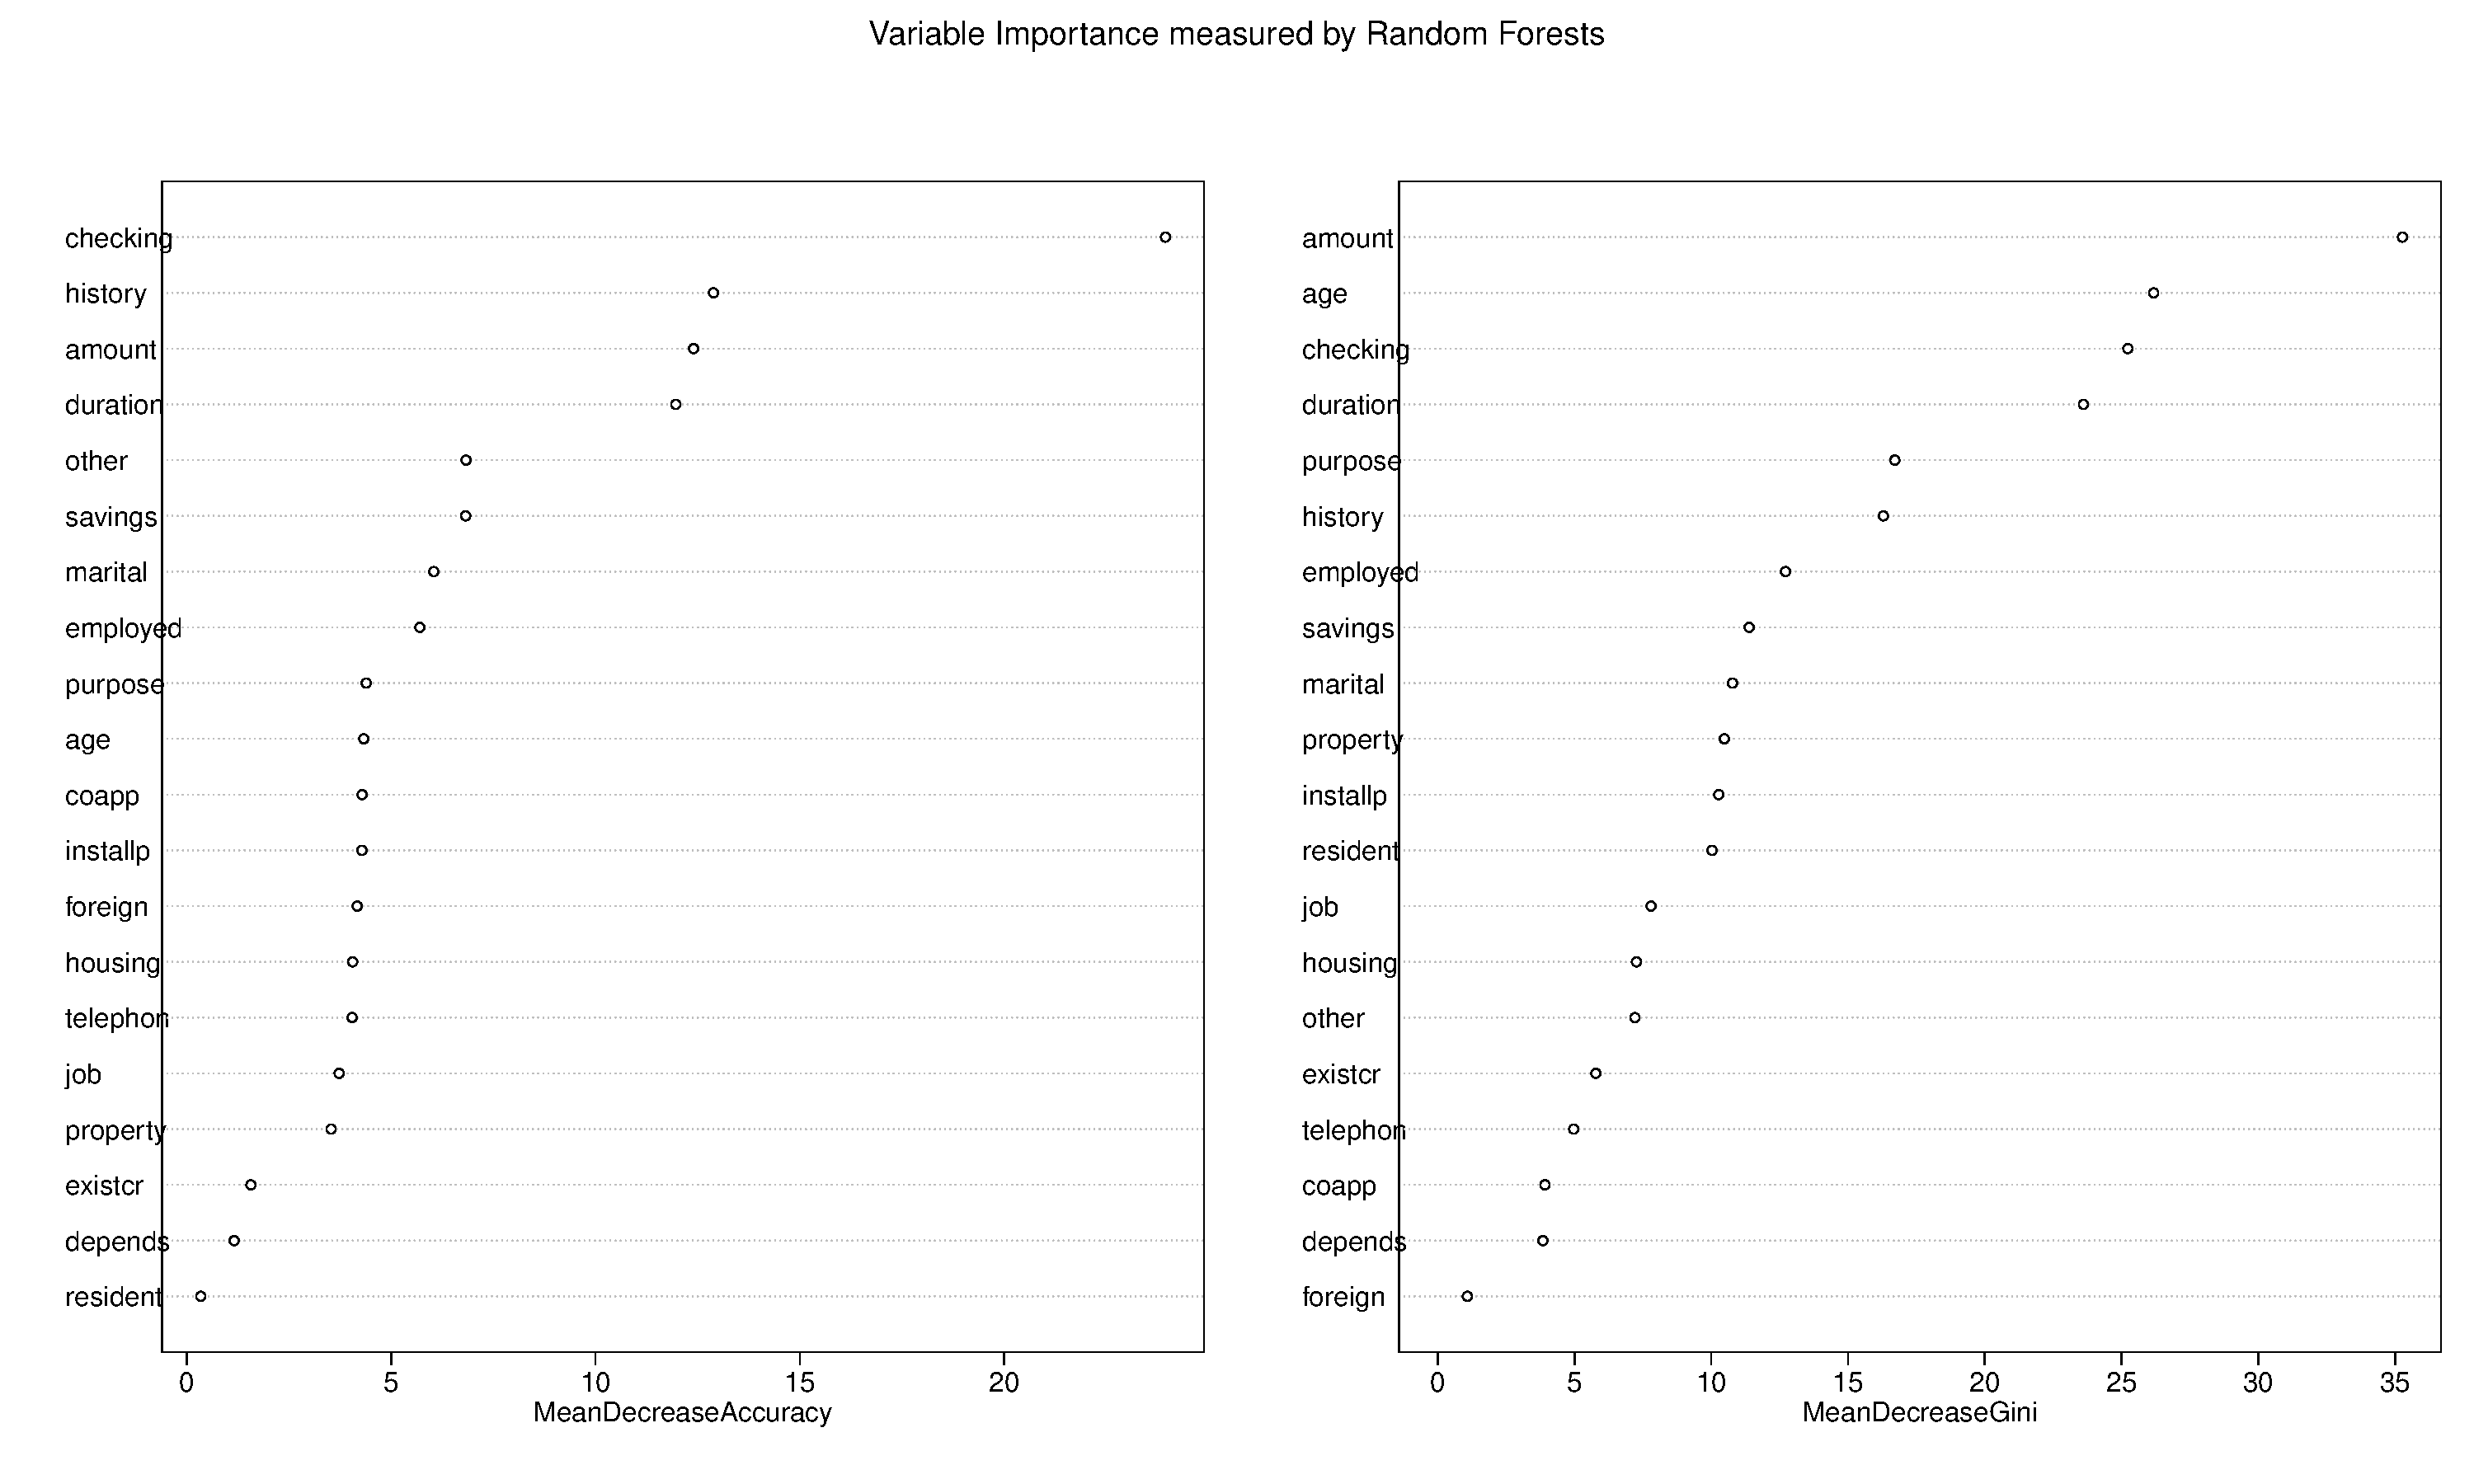
\includegraphics[width=1\linewidth]{varimp.pdf}
\end{figure}
\end{frame}

%------------------------------------------
%\begin{frame}
%\frametitle{Error Rates of Random Forests}
%\begin{figure}
%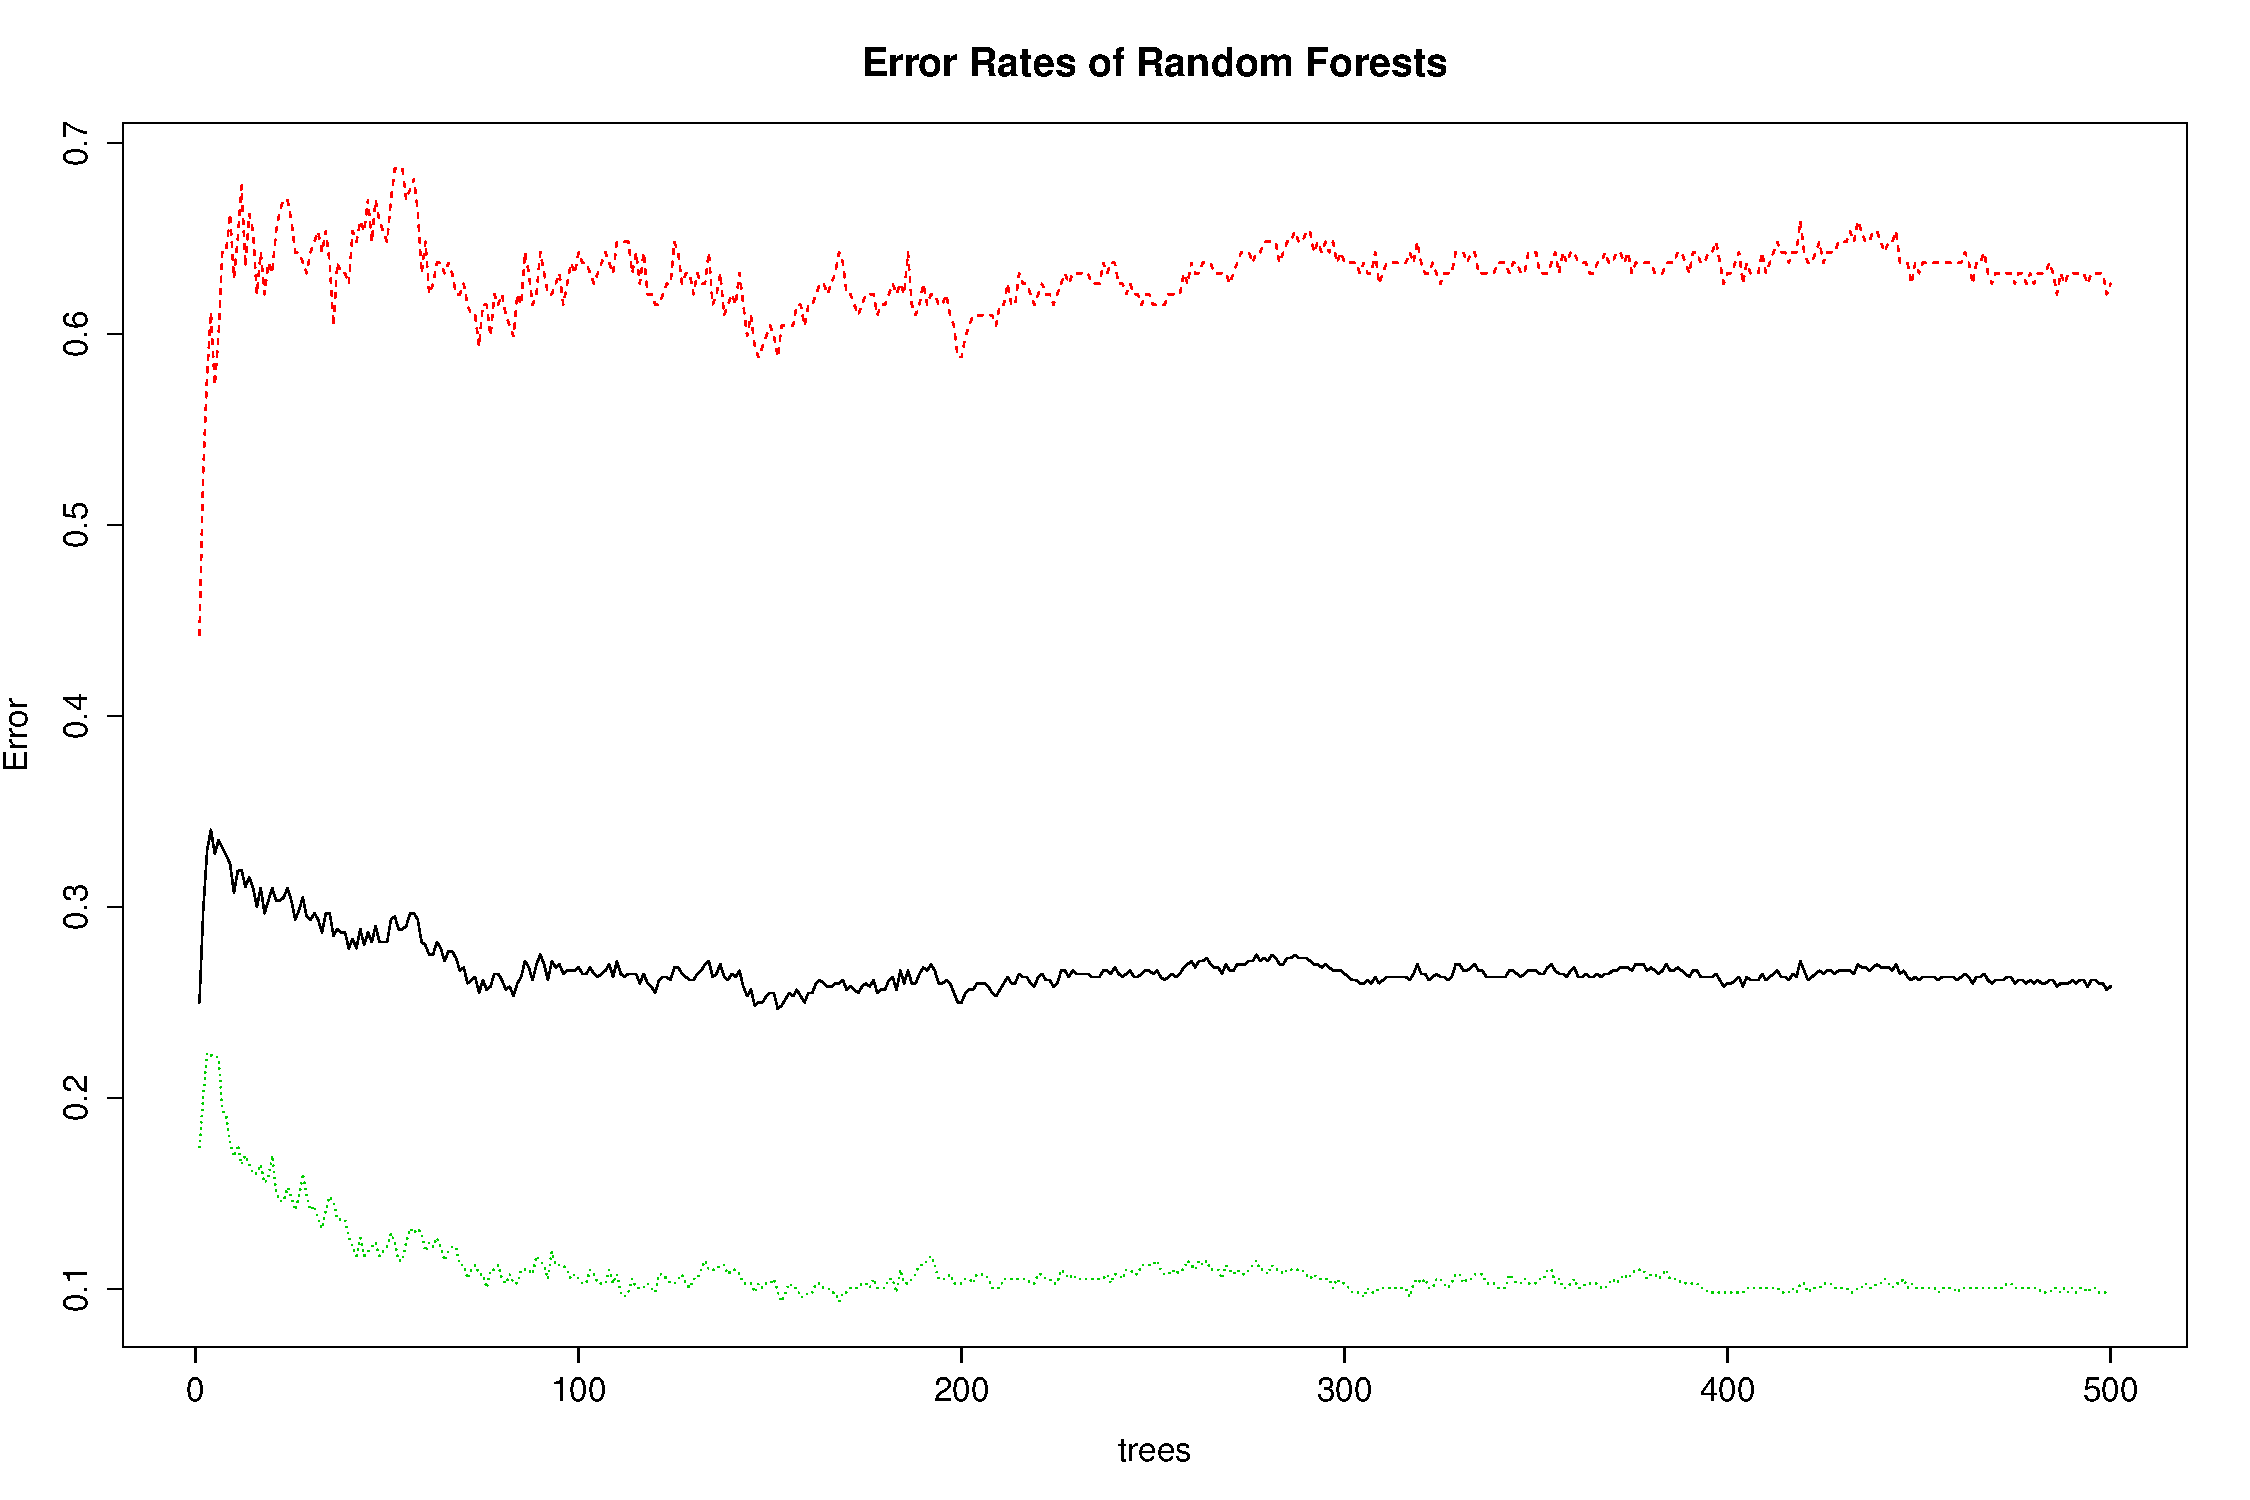
\includegraphics[width=0.8\textwidth]{rferror.pdf}
%\end{figure}
%\end{frame}

\section{performance}
\subsection{performance indicators}
%------------------------------------------
\begin{frame}
Classifiers are build upon training set and their performance is calculated by the test set. The main 
performance indicator includes:
\begin{itemize}
	\item Accuracy: \# of correct predictive results divided by the total \# of data set.
	\item K-S statistic: Mainly used in credit industry.
	\item AUC: Area under an ROC curve.
\end{itemize}
\begin{columns}[c]
\column{0.6\textwidth}
\begin{figure}
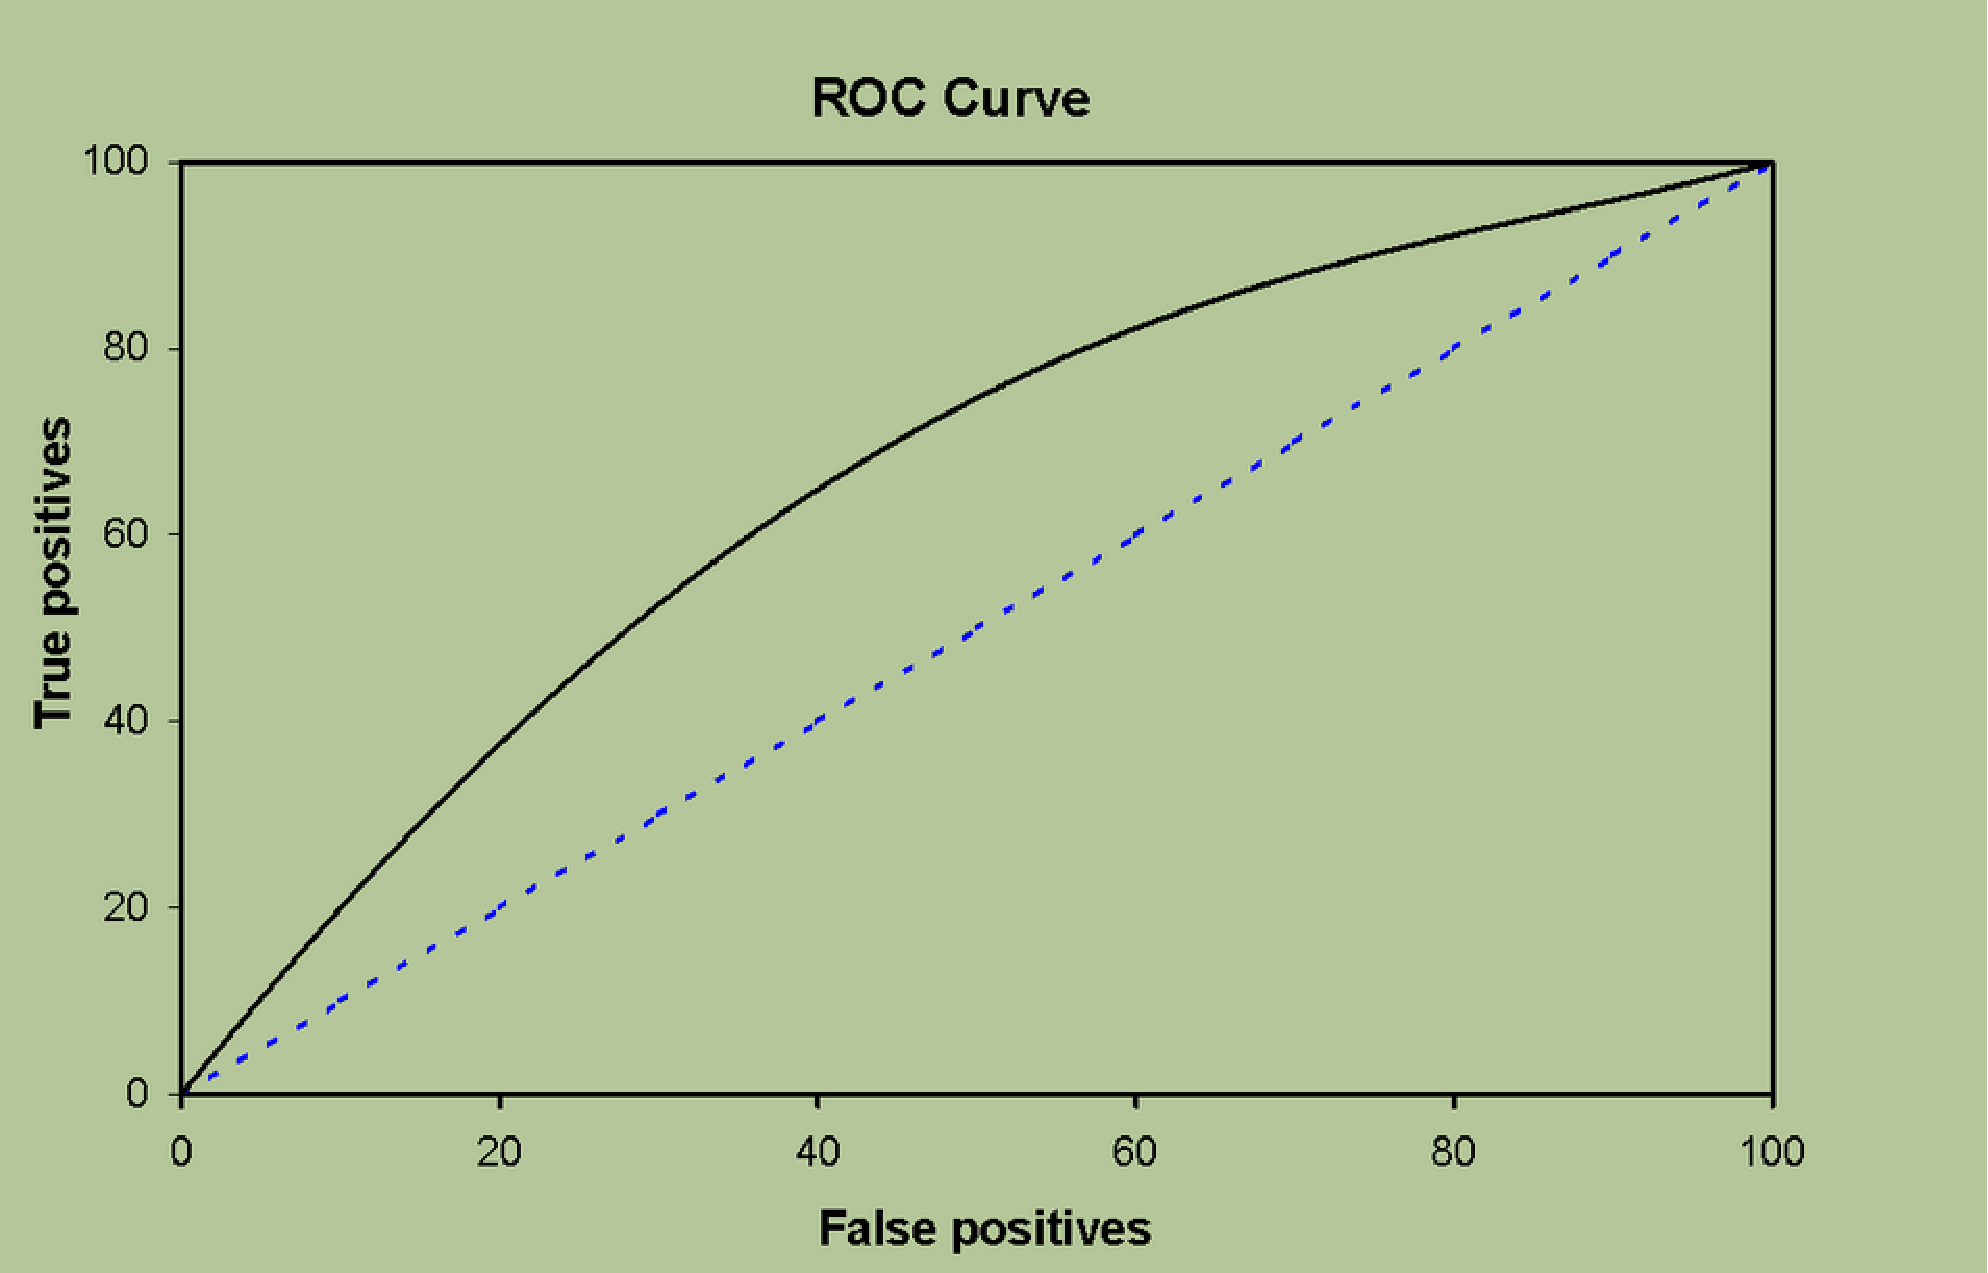
\includegraphics[width=0.8\textwidth]{roc.pdf}
\end{figure}
\column{0.4\textwidth}
\begin{table}[htbp]
  \centering
    \begin{tabular}{rrr}
    \toprule
          & \multicolumn{2}{c}{actual} \\
    \midrule
    \multicolumn{1}{c}{\multirow{2}[0]{*}{predictive}} & TP & FP \\
    \multicolumn{1}{c}{} & FN & TN \\
    \bottomrule
    \end{tabular}%
  \label{tab:roc}%
\end{table}%
\end{columns}
\end{frame}
\subsection{performance results}
%------------------------------------------
\begin{frame}
\frametitle{Performance Results based on German Credit}
\tiny
\begin{columns}[c]
\column{0.5\textwidth}
\begin{figure}
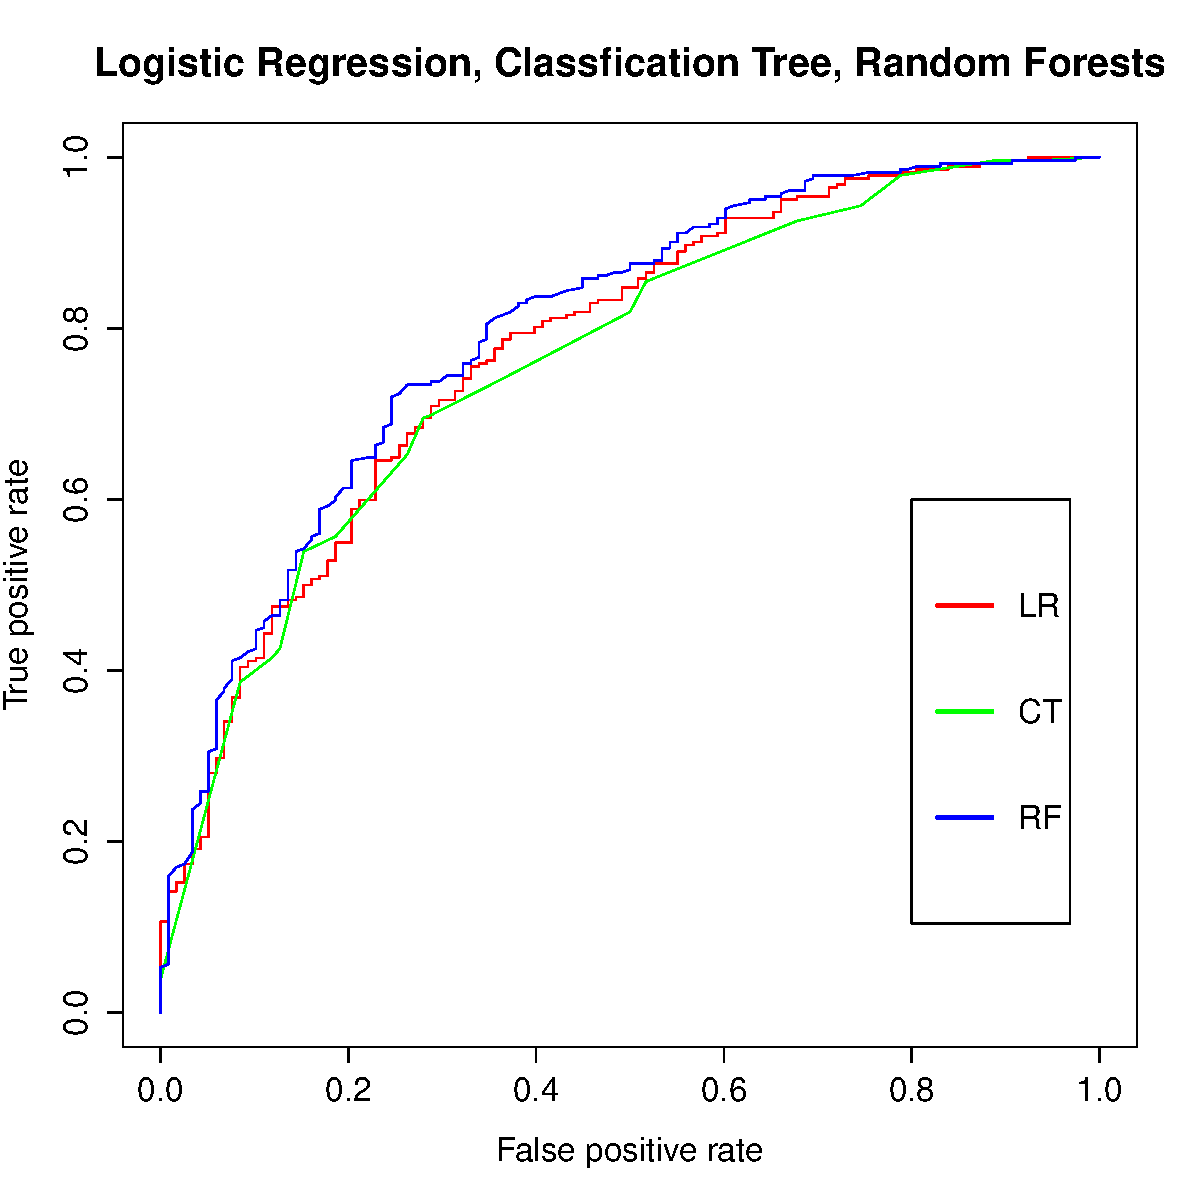
\includegraphics[width=0.9\linewidth]{roc1.pdf}
\end{figure}
\column{0.5\textwidth}
\begin{table}[htbp]
  \centering
  \caption{German Credit}
    \begin{tabular}{lllll}
    \toprule
    Model & KS  & AUC & Accuracy  & Cutoff \\
    \midrule
    LR & 0.425 & 0.776 & 0.773 & 0.421 \\
    CT & 0.415 & 0.762 & 0.753 & 0.250 \\
    RF & 0.474 & 0.798 & 0.780  & 0.472 \\
    \bottomrule
    \end{tabular}%
  \label{tab:roc1}%
\end{table}%
\end{columns}
\end{frame}

\begin{frame}
\frametitle{Performance Results based on Kaggle}
\tiny
\begin{columns}[c]
\column{0.5\textwidth}
\begin{figure}
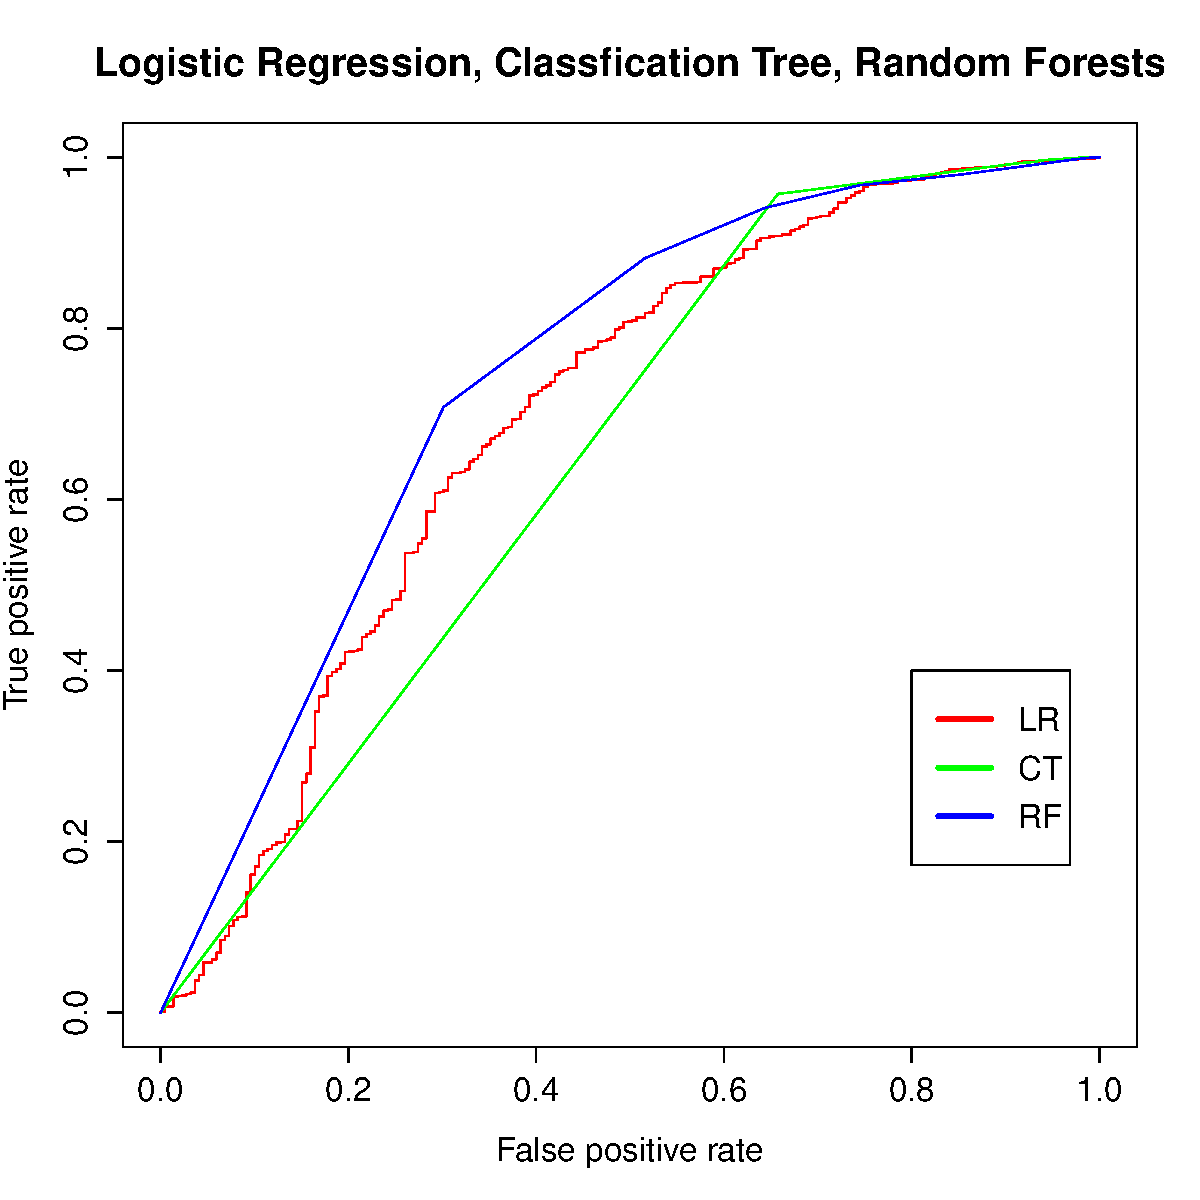
\includegraphics[width=0.9\linewidth]{roc2.pdf}
\end{figure}
\column{0.5\textwidth}
% Table generated by Excel2LaTeX from sheet 'stat2'
\begin{table}[htbp]
  \centering
  \caption{Kaggle}
    \begin{tabular}{lllll}
    \toprule
    Model & KS  & AUC & Accuracy  & Cutoff \\
    \midrule
    LR & 0.329 & 0.695 & 0.933 & 0.727 \\
    CT & 0.300 & 0.651 & 0.933 & 0.308 \\
    RF & 0.407 & 0.741 & 0.932 & 0.300 \\
    \bottomrule
    \end{tabular}%
  \label{tab:roc2}%
\end{table}%

\end{columns}
\end{frame}

\section{conclusions}
%------------------------------------------------
\begin{frame}
\frametitle{Conclusions}
\begin{block}{\#1}
In the light of ROC curve, we can find that random forests have the most extraordinary performance followed 
by logistic regression, and classification tree. 
\end{block}

\begin{block}{\#2}
In comparison with classification tree, random forests illustrates the efficiency and accuracy of ensemble 
learning.
\end{block}

\begin{block}{\#3}
Random forests will reach a higher performance with the help of logistic regression.
\end{block}


\end{frame}


%------------------------------------------------

\begin{frame}
\Huge{\centerline{Thanks!}}
\end{frame}

%----------------------------------------------------------------------------------------

\end{document} 